%!TEX root = ../thesis.tex
%*******************************************************************************
%****************************** Seventh Chapter **********************************
%*******************************************************************************

% **************************** Define Graphics Path **************************
\ifpdf
    \graphicspath{{content/chapter8/figs/raster/}{content/chapter8/figs/pdf/}{content/chapter8/figs/}}
\else
    \graphicspath{{content/chapter8/figs/vector/}{content/chapter8/figs/}}
\fi

\nomenclature[z-nea]{NEA}{North-East Atlantic}
\nomenclature[z-lgcp]{LGCP}{log-Gaussian Cox process}
\nomenclature[z-sdg]{SDG}{Sustainable Development Goal}
\nomenclature[z-emodnet]{EMODnet}{European Marine Observation and Data
Network}
\nomenclature[z-ospar]{OSPAR}{Convention for the Protection of the Marine Environment of the North-East Atlantic}
\nomenclature[z-msfd]{MSFD}{Marine Strategy Framework Directive}
\nomenclature[z-hdi]{HDI}{Highest Density Interval}
\nomenclature[z-ppd]{PPD}{Posterior Predictive Distribution}

% \begin{textquote}
%     Every day, the equivalent of over \num{2000} garbage trucks full of plastic are dumped into our oceans, rivers and lakes. As a result, plastic pollution is set to triple by 2060 if no action is taken.
% \end{textquote}

\part[Pattern Identification in the Scarce Data Regime]{Pattern Identification\\in the Scarce Data Regime}\label{part:scarce_data}

\chapter[A Bayesian Machine Learning Approach to Seasonal Variations in Beach Litter Pollution]{A Bayesian Machine Learning Approach to\\Seasonal Variations in Beach Litter Pollution}\label{chapter:beach_litter}


While the era of Earth observation has resulted in massive datasets propelling advances in fields like weather and climate science \cite{price_probabilistic_2024,chen_machine_2024}, some environmental challenges remain difficult to tackle due to a lack of sufficient data. A prime example is the pervasive issue of global plastic pollution. Despite recent progress in our scientific understanding of this problem\footnote{The political dimension also hinders progress. As of December 2024, negotiators in Busan, South Korea, failed after over two years of talks to finalize a United Nations treaty aimed at significantly reducing plastic pollution \cite{stallard_global_2024}. The main obstacle was differing priorities: some countries seek to limit the production of non-essential plastics, while others, particularly petrochemical producers, prefer to focus on waste management.}, much remains unknown, largely because of extremely limited and scattered observational data. This scarcity presents a significant obstacle to improving our comprehension of the inherent spatio-temporal dynamics of plastics in the environment. Even the most comprehensive large-scale observational datasets rarely exceed a few dozen observations at a given location, making the inference of spatio-temporal trends extremely challenging. Therefore, this problem of pattern identification sits at the lower end of the data density spectrum presented in Chapter~\ref{chapter:intro}.

In this chapter, we tackle the challenge of limited and scattered observational data on plastic pollution by using Gaussian process regression within a Bayesian framework to model its spatio-temporal patterns. This approach allows us to address the scarcity and irregularity of data while enabling statistically robust inferences. We focus specifically on beach litter for two main reasons: (1) monitoring beaches is labor-intensive, leading to particularly scarce data, and (2) beaches tend to accumulate high concentrations of marine litter, making them critical areas of concern. The results presented here have also been published in

\begin{itemize}
    \item \highlightnames{1}{\fullcite{rieger_seasonal_2024}}.
\end{itemize}


This chapter is organized as follows: we begin with a comprehensive overview of the current state of plastic pollution on beaches (Section~\ref{sec:beach_litter:introduction}). Next, we describe the data sets and methods used in our analysis (Section~\ref{sec:beach_litter:methods}). We then present and discuss our findings (Section~\ref{sec:beach_litter:results}) before concluding with final thoughts and implications (Section~\ref{sec:beach_litter:conclusion}).

\section{Plastic Pollution on Beaches}\label{sec:beach_litter:introduction}

Beach litter, predominantly composed of plastics \cite{morales-caselles_inshoreoffshore_2021, lacroix_abundance_2023}, has emerged as a significant environmental challenge, impacting societies globally with its adverse effects on marine ecosystems \cite{chenet_plastic_2021}, wildlife \cite{thiel_impacts_2018,alexiadou_ingestion_2019,barboza_microplastics_2020}, and human health \cite{van_cauwenberghe_microplastics_2014,rochman_anthropogenic_2015}. Since the 1950s, plastic production has surged almost exponentially---from \qtyrange{2}{400}{million~tonnes} annually---with less than \qty{9}{\percent} being recycled and an estimated \qty{23}{\percent} ending up as trash in the environment\footnote{Almost half (\qty{49}{\percent}) of plastic waste is now sent to landfills, and the remaining \qty{19}{\percent} is incinerated \cite{oecd_global_2023}. Over all lifecycle stages, plastics emit about \qty{1.79}{billion~tonnes} of CO$_2$eq, which accounts for \qty{3.3}{\percent} of global greenhouse gas emissions and fuels climate change.} \cite{geyer_production_2017,geyer_production_2020,oecd_global_2023}. Current estimates indicate that marine plastic inputs range between \qtyrange{0.5}{0.7}{million~tonnes} pear year \cite{kaandorp_global_2023, zhang_plastic_2023}, resulting in a standing stock of approximately \qtyrange{3.0}{3.4}{million~tonnes} of marine plastic litter \cite{kaandorp_global_2023}. Plastic litter can now be found everywhere on Earth, from the most isolated islands \cite{imhof_spatial_2017} and remote polar regions \cite{waller_microplastics_2017} to the depths of marine trenches \cite{chiba_human_2018}.

Beaches, despite covering less than \qty{0.02}{\percent} of the global marine environment\footnote{This estimate was calculated by approximating the area of ice-free shorelines: The Earth's total surface area is approximately \qty{510}{million~km^2}, with \qty{361}{million~km^2} (\qty{70.8}{\percent}) covered by water. According to \citet{luijendijk_state_2018}, the total length of ice-free shorelines is about \qty{1.11}{million~km}. Assuming an average beach width of \qty{50}{meters}, the area of beaches is calculated as $\qty{1.11}{million~km} \times \qty{0.05}{km} = \qty{55500}{km^2}$, which is roughly \qty{0.015}{\percent} of the global marine environment. This estimate likely overstates the area of sandy beaches, as they constitute only about one-third of all shorelines \cite{luijendijk_state_2018}.}, likely accumulate up to \qty{2}{\percent} of global marine plastics \cite{kaandorp_global_2023}. This leads to relatively high concentrations of pollution in these areas compared to other parts of the marine environment. Recent studies suggest a balanced contribution of plastic pollution from land-based activities and marine sources, particularly from fishing-related activities, each accounting for about half of the total \cite{li_plastic_2016,kaandorp_global_2023}. Concurrently, aquaculture production has witnessed significant growth \cite{paolo_satellite_2024,fao_state_2022}, now accounting for \qty{50}{\percent} of global fish production \cite{fao_state_2022}, and increasingly contributes to marine pollution \cite{bringer_coastal_2021,lin_environmental_2023,kruger_plastic_2020,hinojosa_floating_2009}.

Although much progress has been made in understanding how and where plastics accumulate in our marine environment \cite[e.g.][]{strokal_river_2023,mai_country-specific_2023,morales-caselles_inshoreoffshore_2021,chassignet_tracking_2021}, many open questions remain regarding their spatio-temporal variations. One of the main reasons for this is the lack of sufficient and consistent observational data \cite{haarr_global_2022}. Most of the data available today---from lakes, rivers, beaches, and the open ocean---are based on in situ measurements. These are often costly in terms of time and resources, resulting in a very sparse set of observations. Additionally, due to a lack of standardized survey protocols, not all globally available data are easily comparable.

Beach litter observations remain particularly scarce as they mostly rely on cumbersome in situ surveys, which are difficult to automate. While remote sensing of beach litter using unmanned aerial vehicles such as drones combined with machine learning classification has been demonstrated as a more efficient method to survey beach litter (see, for instance, \citet{goncalves_beach_2022} and references therein for advances in this direction), this approach is still under development. For the open ocean, it was recently shown that it is possible to measure plastic pollution---which often forms large coherent structures or filaments---using satellites \cite{cozar_proof_2024}, marking a major step forward. Unfortunately, applying the same approach to beach litter is challenging due to the need for much higher resolution imagery.

Seasonal variations in beach litter present a complex picture, with various studies reporting differing peak pollution periods across seasons \cite{gago_characteristics_2014,declerck_transport_2019,schulz_multi-criteria_2013,ruiz_modelling_2022,watts_through_2017,asensio-montesinos_seasonal_2019,ruiz_modelling_2022,rios_spatio-temporal_2018,williams_beach_2017}. A consistent large-scale seasonal pattern remains elusive \cite{schulz_multi-criteria_2013,nelms_marine_2017}, possibly because of insufficient survey data \cite{schulz_baseline_2019, haarr_global_2022}. Improved understanding of beach litter seasonality is vital for identifying anthropogenic sources and setting effective, evidence-based management policies. Notably, seasonality in plastic emissions has been observed from riverine discharges \cite{lebreton_river_2017,van_emmerik_seasonality_2019, van_emmerik_river_2023} and capture fisheries \cite{kroodsma_tracking_2018,paolo_satellite_2024}, while the seasonal dynamics of marine aquaculture (mariculture) contributions are less documented. The anticipated rise in global plastic waste and seafood demand \cite{lebreton_future_2019, fredheim_future_2018}, driven by population growth and socioeconomic factors, underscores the necessity to explore these seasonal dynamics comprehensively.

In this study, we aim to (1) investigate the seasonal variations of anthropogenic beach litter, (2) identify regions where these variations are particularly pronounced---referred to as `seasonal hotspots', and (3) understand the underlying drivers. Focusing on the North-East Atlantic (NEA), we utilize the OSPAR dataset \cite{ospar_comission_convention_1992}, one of the most comprehensive in-situ beach litter datasets globally. Despite its extensive coverage, the infrequent surveys of many beaches present challenges in detecting statistically significant seasonality \cite{schulz_multi-criteria_2013,schulz_baseline_2019,grundlehner_towards_2023}. Therefore, we employ a spatial log-Gaussian Cox process \cite{diggle_bivariate_1983,moller_log_1998} to model macroplastic distributions, leveraging its Bayesian machine learning framework to capture complex spatial patterns while allowing robust statistical inference. This approach enables us to more accurately model probability distributions of beach litter by incorporating information from nearby beaches and exploiting spatial autocorrelation patterns \cite{grundlehner_towards_2023}.

This study seeks to enrich the discourse on sustainable, evidence-based management strategies for beach litter \cite{likens_role_2010,van_loon_european_2020}, aligning with the EU's Marine Strategy Framework Directive (MSFD) and directly supporting the marine litter objectives outlined in the OSPAR North-East Atlantic Environment Strategy 2030 \cite{ospar_comission_strategy_2021}. By providing insights into the seasonal dynamics and sources of beach litter, our research underscores the need for targeted actions to prevent and significantly reduce marine litter inputs, in line with OSPAR's Strategic Objective 4. While our focus is regional, these efforts also contribute to broader Sustainable Development Goals (SDGs), mainly related to marine life conservation (SDG 14). Furthermore, as macroplastics are a major source of microplastics entering the marine environment \cite{strokal_river_2023}, better management and mitigation of macroplastic emissions can support efforts regarding good health (SDG 3) and clean water (SDG 6).


\section{Materials \& Methods}\label{sec:beach_litter:methods}
Throughout this work, we define the seasons as follows: winter (December to February), spring (March to May), summer (June to August), and autumn (September to November). Following previous OSPAR data assessments \cite{lacroix_abundance_2023}, macroplastics are defined as artificial polymer materials larger than 2.5 cm. In this manuscript we use the term beach litter interchangeably with macroplastics.

\subsection{Beach Litter Data}\label{sec:methods:ospar}
We utilized the OSPAR dataset \cite{ospar_comission_convention_1992,lacroix_abundance_2023}, comprising 4,305 surveys. Our regional focus is on the North-East Atlantic (NEA), specifically the Atlantic coastlines of Belgium, Denmark, France, Germany, Ireland, the Netherlands, Norway, Portugal, Spain, Sweden, and the United Kingdom. This area closely aligns with OSPAR maritime regions II (Greater North Sea), III (Celtic Seas), and IV (Bay of Biscay and Iberian Coast) but differs slightly from the official OSPAR definition of the NEA.

Specifically, we excluded overseas regions such as the Azores, the Canary Islands, the Faroe Islands, and Greenland, as well as areas above 65º north latitude and data from the Mediterranean Sea, to maintain a consistent geographic scope. Our focus on this specific subregion is motivated by data availability and considerations of spatial scale and model complexity. Regions like Greenland and Iceland were excluded due to limited seasonal coverage, with surveys predominantly conducted during summer and autumn, making it challenging to establish seasonal differences throughout the year. Additionally, including remote areas would introduce larger spatial scales, requiring modifications to our model that could increase complexity without significant benefit from the limited additional data.

Entries where external cleanups may have been performed before the OSPAR survey, as noted in the `Survey: Remarks' category, were excluded. For surveys deviating from the standard 100-meter length, we extrapolated beach litter counts when the actual survey length was provided; otherwise, these surveys were excluded. We then aggregated all OSPAR categories of artificial polymer materials larger than 2.5 cm (macroplastics) into a common category \cite{lacroix_abundance_2023}. 

According to the OSPAR survey guidelines \cite{wenneker_guideline_2010}, beaches are surveyed quarterly, specifically in January, April, July, and October. We identified 87 instances of multiple surveys per season for the same beach and year; to mitigate sample frequency bias in beach litter detection \cite{ryan_effect_2014}, we selected the maximum litter item count from these surveys for each season, beach, and year. The refined dataset comprised 3,866 surveys from 168 beaches, documenting over 2 million items.

We estimated the number of items originating from land-based, fishing-related and mariculture-related activities, including only categories that are relatively unambiguous. For mariculture-related items, we used OSPAR categories explicitly linked to mariculture \cite{skirtun_plastic_2022} (OSPAR IDs 28, 29, 30 and 114). Fishing-related activities were based on the SEA category \cite{lacroix_abundance_2023}, excluding items associated with mariculture and ambiguous items like strings \cite{skirtun_plastic_2022}. Land-based items were defined by the residual categories, excluding all generic categories (OSPAR IDs 46, 47 and 48). As a result, $39.9\%$ of items within the preprocessed OSPAR dataset could be assigned to either land, fishing or mariculture.



\subsection{Log-Gaussian Cox process model}\label{sec:methods:LGCP}
We utilized a log-Gaussian Cox process (LGCP) \cite{moller_log_1998} in this study to map the spatial distribution and intensity of macroplastic beach litter. In the LGCP framework, the logarithm of the intensity function is modeled as a Gaussian process ($\mathcal{GP}$) \cite{bishop_pattern_2006}, making it particularly suitable for environmental and ecological data exhibiting spatial dependence. 

The observed over-dispersion in the beach litter data (Supplementary Figure~11), where the variance exceeds the mean, necessitated adapting the LGCP to use a Negative Binomial distribution instead of the traditional Poisson distribution. The Negative Binomial distribution effectively models count data with over-dispersion. The over-dispersion parameter $\phi$ modulates the variance independently of the mean, capturing the inherent variability in litter quantities.

Let $Y$ denote the macroplastic counts, assumed to follow a Negative Binomial distribution with mean $\mu$ and over-dispersion parameter $\phi$:

\begin{align}
    Y &\sim \mathcal{NB} (\mu, \phi).
\end{align}

The mean $\mu$ is linked to spatial covariates (longitude and latitude of each beach) through a Gaussian process after applying a Yeo-Johnson transformation \cite{yeo_new_2000} $\mathcal{T}$:

\begin{align}
    \mathcal{T}(\mu) &\sim \mathcal{GP}(\mu_{\mu}, K)
\end{align}

The Yeo-Johnson transformation, accommodating both positive and zero-valued data, ensures positivity and adaptability to the data's skewness:

\begin{align}
    \mathcal{T}(x) = \begin{cases}
      ((x+1)^{\lambda} - 1) / \lambda  & \lambda \neq 0,\\
      \ln x + 1 & \lambda = 0.
\end{cases}    
\end{align}

The parameter $\lambda$ was estimated via maximum likelihood estimation using all beaches and seasons, resulting in $\lambda = 4.27 \times 10^{-3} \approx 0$.

The covariance function $K$ of the $\mathcal{GP}$ models the spatial correlation. A combination of two Matérn $3/2$ kernels \cite{williams_gaussian_2006} was chosen to capture different scales of spatial dependence:

\begin{align}
    k(b,b') &= k_1^{\left[3/2\right]}(b, b') + k_2^{\left[3/2\right]}(b, b'),
\end{align} where 
\begin{align}
    k_i^{\left[3/2\right]}(b, b') &= \eta_i^2 \left(1 +  \frac{\sqrt{3}d}{\rho_i} \right) \exp \left(- \frac{\sqrt{3}d}{\rho_i} \right), \, i=1,2.
\end{align}

Here, $\eta_i$ and $\rho_i$ represent the variance and spatial scale parameters of the kernels, and $d$ denotes the chordal distance \cite{jeong_spherical_2017} between locations $b$ and $b'$. The parameters $\rho_i$ define the typical length scales over which spatial autocorrelation occurs, while $\eta_i$ modulate the amplitude of these correlations.

Prior distributions were specified for all model hyperparameters to reflect underlying assumptions and ensure robust model inference. For the mean function $\mu_{\mu}$ of the GP, a weakly informative prior $\mu_{\mu} \sim \mathcal{N}(\alpha, \beta)$ was selected. The parameters $\alpha$ and $\beta$ were defined such that the \qty{95}{\percent} highest density interval (HDI) of the prior encompasses the 2.5\textsuperscript{th} and 97.5\textsuperscript{th} percentiles of the average beach litter densities, $\left[\mathcal{T}(q_{0.025}), \mathcal{T}(q_{0.975})\right]$, determined from the data. This range includes previously estimated median pollution levels of 149 \cite{hanke_eu_2019} and 252 \cite{lacroix_abundance_2023} items per 100 meters of beachline.

For the length scales $\rho_i$, positive-valued Inverse Gamma distributions $\rho_i \sim \mathcal{IG}(\gamma_i, \delta_i)$ were used. The hyperparameters $\gamma_i$ and $\delta_i$ were defined such that the \qty{95}{\percent} HDIs extend from 10 to 100 km for short length scales ($i=1$) and from 100 to 5,000 km for medium-to-long length scales ($i=2$), effectively capturing different spatial autocorrelation ranges.

Weakly informative Gamma priors $\eta_i \sim \mathcal{G}(\epsilon_i, \kappa_i)$ were set for the variance parameters. The parameters $\epsilon_i$ and $\kappa_i$ were defined such that the \qty{95}{\percent} HDIs cover the interval $\left[1/\sqrt{2}, 2/(3\sqrt{2})\right]$. This configuration, determined via exploratory prior predictive checks, ensures the $\mathcal{GP}\text{'s}$ uncertainty covers the entire range of possible values in the Yeo-Johnson transformed data space, providing the model with flexibility in determining the relative contribution of each length scale to the autocovariance function.

For the over-dispersion parameter $\phi$, a weakly informative Inverse Gamma distribution $\phi \sim \mathcal{IG}(\nu, \sigma)$ was set, with $\nu$ and $\sigma$ defined such that the \qty{95}{\percent} HDI covers $\left[2, 9\right]$. This is consistent with observed ranges of over-dispersion in the data (Supplementary Figure~11).

The model was fitted using the No-U-Turn Sampler \cite{hoffman_no-u-turn_2014} (NUTS), a variant of Hamiltonian Monte Carlo, chosen for its efficiency in handling high-dimensional parameter spaces and its ability to navigate complex posterior landscapes. Four chains were run, each with 9,000 iterations, discarding the first 8,000 iterations as warm-up.

Convergence of the model parameters to a stationary distribution was verified by inspecting trace plots and using the $\hat{R}$ statistic \cite{gelman_inference_1992}, which was below 1.05 for all parameters. Comparison between prior and posterior distributions of the LGCP model hyperparameters (Supplementary Figure~12) confirmed appropriate updating of beliefs in light of the data.

Posterior predictive checks were performed for all beaches by comparing the modeled mean and variance of each beach to its sample statistics (Supplementary Figure~13), revealing generally good agreement. This indicates that the model adequately captures the underlying data structure, validating its suitability for predicting macroplastic distributions.

\subsection{LGPC Model Posterior Inference}\label{sec:methods:inference}
The seasonal effect size ($\sigma$) quantifies the degree of difference in macroplastic densities between seasons, ranging from $-1$ to $1$. Values near $-1$ or $1$ indicate substantial seasonal differences, while a value of zero suggests no difference.

For any two distinct seasons $s$ and $s'$ from the set $\{\text{Winter, Spring, Summer, Autumn}\}$, let $Y$ and $Y'$ represent the macroplastic densities with posterior predictive distributions $p(y|D)$ and $p(y'|D')$, based on survey data $D$ and $D'$. The effect size between these seasons is calculated as the probability that the density in season $s$ exceeds that in season $s'$:

\begin{align}
    \hat{\sigma}_{s, s'} &= p(y>y'|D,D') \nonumber\\
    &= \int_{\mu}\int_{\mu'} I(\mu > \mu') p(y, y' | D, D') \dd{s}\dd{s'}    
\end{align} 

where $I(y > y')$ is an indicator function equal to $1$ when $y > y'$ and $0$ otherwise.

To normalize this measure between $-1$ and $1$, we compute:

\begin{align}
    \sigma_{s,s'} = 2\hat{\sigma}_{s,s'} - 1.
\end{align}

The overall seasonal effect size $\sigma$ is then defined as the maximum absolute value among all season pairs:

\begin{align}
    \sigma = \max_{s \neq s'} \left| \sigma_{s, s'} \right|.
\end{align}


Statistical confidence ($\gamma$) measures the likelihood that the observed seasonal differences in mean macroplastic densities are statistically significant. For mean densities $\mu$ and $\mu'$ in seasons $s$ and $s'$, with posterior distributions $p(\mu)$ and $p(\mu')$, we determine the highest density intervals (HDIs) at a confidence level $c \in [0, 1]$ for each.

The statistical confidence is then given as the maximum confidence level $c$ such that the HDIs of $\mu$ and $\mu'$ do not overlap:

\begin{align}
    \gamma = \max \{c \, | \, \text{HDI}_{\mu}(c) \cap \text{HDI}_{\mu'}(c) = \emptyset \}.
\end{align}

\subsection{Clustering of Seasonal Patterns}\label{sec:methods:clustering}
Principal Component Analysis (PCA) serves as a fuzzy clustering method \cite{drineas_clustering_2004} to discern beaches with analogous seasonal macroplastic patterns. Utilizing the posterior predictive distributions (PPD) from the seasonal LGCP models, we systematically analyze the data as follows:
\begin{enumerate}
    \item \textbf{Matrix representation:} Define $Y \in \mathrm{N}^{(n_b \times n_s)}$ as a matrix of realizations for $n_b=168$ beaches across $n_s=4$ seasons, drawn from the PPD. Here, $y_{bs}$ denotes the modeled macroplastic density for beach $b$ in season $s$.
    \item \textbf{Normalization:} To compare seasonal distributions equitably, we normalize each beach's macroplastic counts by its annual total, resulting in relative seasonal shares:

    \begin{align}
    \hat{y}_{bs} = \frac{y_{bs}}{\sum_s y_{bs}}    
    \end{align}
    
    \item \textbf{Weighted PCA:} Implementing weighed PCA on the normalized matrix $\hat{Y}$ allows for the accentuation of seasonal covariance, using beach-specific statistical confidence $\gamma_b$ as weights. PCA yields eigenvalues $\lambda_i$, eigenvectors $v_i$ and corresponding principal component (PC) scores, segregating the data into clusters based on sign. Each eigenvector reflects a distinct cluster, separated into positive and negative parts:

    \begin{align}
    \nu_i^+ = \sum_{v_{bi} > 0} v_{bi}^2, \qquad \nu_i^- = \sum_{v_{bi} < 0} v_{bi}^2
    \end{align}
    
    where $\nu_i^+/\nu_i^-$ quantifies the explained variance by positive/negative clusters, respectively, offering insight into their respective contributions to the overall seasonal variance in macroplastic distribution.
\end{enumerate}

We perform these steps for $N=4000$ realizations drawn from the PPD so that we obtain distributions for all quantities. The degree of membership of beach $b$ to cluster $i$ is then given by the mean of the distribution of $v_{ib}$. The associated statistical confidence is given by the fraction of the distribution being above/below 0, renormalized to be between 0 and 1 to ensure a proper probability. For instance, the statistical confidence of the positive clusters read

\begin{align}
\gamma_{ib} = \frac{2}{N} \sum_{j}^N I(v_{ib} > 0) - 1,
\end{align}

where $I(\cdot)$ is the indicator function.

Supplementary Figure~14 shows that the first two clusters, cluster $C1^+$ and $C2^+$, are statistically significant and explain over 50\% of the variance.



\subsection{Sources of Macroplastics and Seasonal Potential}\label{sec:methods:seasonal_potential}

We analyzed riverine emissions (A), fisheries (B), and mariculture activities (C) to understand their potential impact (D) on seasonal beach litter patterns.

(A) High-resolution, 6-hourly river discharge data from 2010 to 2020 were averaged into monthly means to create climatologies. Macroplastic emissions from rivers were inferred using model data on mismanaged solid waste exports to the sea \cite{strokal_river_2023}. We scaled the data from annual to monthly emissions based on river discharge under the assumption of proportionality. While this simplification does not capture the full complexity of riverine macroplastic emissions \cite{van_emmerik_seasonality_2019}, it provides a reasonable approximation for understanding seasonal emissions patterns \cite{lebreton_river_2017, cheung_seasonal_2016,van_emmerik_hydrology_2022,cozar_proof_2024}, excluding extreme events \cite{van_emmerik_river_2023}.

(B) We utilized fishing intensity data from the Global Fishing Watch dataset \cite{kroodsma_tracking_2018}, spanning from 2013 to 2020, transformed into a gridded format on a regular \ang{0.25} longitude-latitude grid. To reduce dimensionality, we aggregated the high-resolution spatial data into predefined regions based on ocean basins from NaturalEarth (1:50 million scale) and extended these regions based on oceanographic settings (Figure~\ref{fig05}). The regions include the Bay of Biscay (0), North Sea (1), Irish Sea (2), English Channel (3), Bristol Channel (4), Inner Seas (5), Skagerrak (6), West Iberian Sea (7), Gulf of Cadiz (8), West Irish Sea (9), and South Irish Sea (10). Monthly climatologies of fishing intensity were calculated for each of these 11 regions.

(C) To estimate plastic emissions from mariculture, we assumed local emission rates are proportional to production intensity. We used a global dataset of mariculture production sites \cite{clawson_mapping_2022}, which partially relies on data from the European Marine Observation and Data Network (EMODnet) \cite{emodnet_emodnet_2014,emodnet_emodnet_2021}. The EMODnet dataset distinguishes between individual farms and production areas, unlike the global dataset. 

To mitigate potential biases due to differing definitions, we consolidated all locations into production areas by applying a threshold distance below which farms are considered part of a single production area. We estimated this threshold distance by analyzing the distribution of distances between mariculture sites in France, where sites are exclusively production areas in the EMODnet dataset. Histograms of great circle distances revealed that distances below \qty{3}{km} are uncommon in France but prevalent elsewhere, suggesting \qty{3}{km} as the typical minimal separation between production areas. Using this threshold (approximately \ang{0.027} at the equator), we created a regular \ang{0.027} longitude-latitude grid, marking cells with at least one location. For visualization, we aggregated production areas into \ang{0.54} $\times$ \ang{0.54} cells, weighting each grid cell by the cosine of its latitude to account for decreasing cell areas toward the poles. This process refined the mariculture dataset, reducing biases from differing location definitions. 

To estimate seasonal variations in plastic emissions from mariculture, we considered how plastics enter the marine environment. Studies have identified pathways including routine operations, inadequate management, deliberate discharge, and extreme weather \cite{skirtun_plastic_2022, tian_can_2022, global_ghost_gear_initiative_best_2021}, with extreme weather being a significant source in the Northeast Atlantic (NEA) region. While routine emissions likely occur year-round, we hypothesize increased activities -- and thus potential emissions -- during harvest periods.

We proposed two scenarios:

\begin{enumerate}
    \item Adverse weather scenario: Emissions are driven by adverse weather conditions. Monthly plastic emissions rates were assumed proportional to monthly mean ocean wave energy. We obtained monthly climatologies of significant wave height  from the Global Waves Reanalysis \cite{eu_copernicus_marine_service_information_cmems_global_nodate} (2013-2020) and calculated wave energy as the square of the significant wave height. Each production area's monthly climatology was assigned based on the spatial average of wave energies within a \ang{0.5} $\times$ \ang{0.5}rectangle centered on it. The climatology was normalized to an annual average of one and scaled by production area density.
    \item Seasonal activity scenario: Emissions increase during harvest periods. We analyzed approximately 4 million export transaction from 2009 to 2023 obtained from the European Market Observatory for Fishery and Aquaculture Products \cite{eumofa_exports_2024} (EUMOFA) to approximate harvest seasons. Although the export data do not distinguish between fisheries and aquaculture products, the main aquaculture species in the NEA region--salmon (\qty{65}{\percent}), oysters/mussels (\qty{21}{\percent}), and trout (\qty{9}{\percent}) \cite{fao_global_2024}--are predominantly farmed (over \qty{98}{\percent}). 
    
    Our methodology involved several steps. First, we summed export transaction to calculate total monthly exports per species and country. We then removed long-term trends by applying a convolution filter to detrend the data. Next, we determined the seasonal component by averaging the detrended data over all years, weighted by annual export volumes. To compute species-weighted averages, we matched species group in the mariculture dataset \cite{clawson_mapping_2022} and used the min-max-normalized seasonal components weighted by the overall mean annual aquaculture production of individual species. To calculate the mean annual aquaculture production for each species, we used a species-year-weighted average over the years 2001-2020, weighting each year by the number of OSPAR surveys per year and country to account for sampling bias and production increases over time. This process resulted in a seasonal component for each species group and country. Finally, we assigned the seasonal component to each production area based on its proximity to the nearest country and scaled it by production area density.
\end{enumerate}

A third scenario considered river discharge variations, relevant for countries like Portugal where mariculture sites are situated within river mouths \cite{rocha_global_2022}. Seasonal variations were computed similarly to the adverse weather scenario but using river discharge climatologies.

(D) To assess how well river discharges, and fisheries and mariculture explain seasonal beach litter patterns, we calculated the coefficient of variation ($c_{\text{v}}$) to measure seasonal amplitude and the Pearson correlation coefficient ($c_{\text{r}}$) to assess pattern alignment. We adjusted seasons to match the timing of beach litter surveys, shifting them by one month due to the OSPAR sampling protocol prioritizing mid-season surveys--over \qty{70}{\percent} occurred in January, April, July and October. Therefore, we considered November - January, February - April, May - July and August - October for comparisons. The seasonal potential, defined as $\Phi = \max \left( 0, c_{\text{r}} \cdot c_{\text{v}}\right)$, identifies the strongest seasonal signals in potential sources, prioritizing those with considerable variability and temporal alignment with the observed litter patterns.


\section{Results and Discussion}\label{sec:beach_litter:results}


\subsection{Seasonal Variations of Anthropogenic Beach Litter in the North-East Atlantic}


ur analysis, utilizing 3866 surveys from the OSPAR dataset over two decades (2001 - 2020) and encompassing 168 beaches along the western European coastlines, employs a spatial LGCP model (Methods \ref{sec:methods}) to evaluate macroplastic pollution across the four seasons: winter, spring, summer and autumn. Macroplastic pollution was defined as the number of all artificial polymer materials larger than 2.5 cm per 100m of beach length (Methods~\ref{sec:methods:ospar}). We found that median macroplastic levels peak in spring, reaching 232 items per 100 meters of beachline (\itm), with a 95\% Bayesian credible interval (CI) ranging from 79 to 440 \itm. Pollution levels are slightly lower in winter (184 \itm), autumn (174 \itm) and summer (154 \itm), although the broad CIs suggest these differences are not statistically significant (Supplementary Table~1). These results are consistent with previously estimated annual medians for this region  \cite{hanke_eu_2019,lacroix_abundance_2023}.

A more detailed per-beach analysis reveals distinct interseasonal variations in macroplastic pollution, with 15\% of beaches exhibiting such differences at a 95\% confidence level (Figure~\ref{fig01}, Methods~\ref{sec:methods:inference}) increasing to 39\% when the confidence threshold is adjusted to 80\%. 

Further examination of seasonal variation patterns (Figure~\ref{fig02}A) shows that the most common scenario, observed in 36\% of confidence-weighted beaches, involves increased plastic litter in spring compared to summer. Conversely, increased summer litter over spring is the least common scenario, observed in only 9\% of cases. These variations highlight the complex and diverse seasonal patterns of beach litter with a general trend for higher litter accumulation in winter/spring compared to summer/autumn. Among beaches exhibiting seasonal variations, a dominant pattern emerges where winter and spring seasons experience 95\% to 118\% more plastic pollution than the summer and autumn seasons (Figure\ref{fig02}~B). In contrast, beaches following a summer/autumn $>$ winter/spring pattern show a smaller increase, ranging from 60\% to 78\% more macroplastics. The substantial range of confidence intervals for these estimates suggests only weak statistical support for the idea that relative differences are stronger in one season compared to another (Supplementary Table~2).

These findings are consistent with a growing body of scientific evidence showing pronounced seasonal variations of beach litter across various beaches worldwide \cite{cheung_seasonal_2016,simeonova_seasonal_2017,pelamatti_seasonal_2019,orthodoxou_seasonal_2022}, particularly in the NEA region \cite{gago_characteristics_2014,declerck_transport_2019,schulz_multi-criteria_2013,ruiz_modelling_2022,watts_through_2017,asensio-montesinos_seasonal_2019,rios_spatio-temporal_2018}, although a clear large-scale pattern remains elusive. For example, two regional but weak patterns were reported \cite{schulz_multi-criteria_2013} exhibiting an increase in autumn/winter pollution in the wider Atlantic region and a spring peak specifically in the North Sea. In contrast, a comprehensive study focusing on UK beaches found no pronounced seasonal patterns \cite{nelms_marine_2017}. The discrepancy may stem from the insufficient statistical power of both studies. The neighborhood-aware LGCP model approach in our study allows better estimations of litter distributions for each beach by taking into account pollution levels from beaches nearby. Our model suggests that 60\% to 77\% of beaches, depending on the season, in the OSPAR dataset provide useful information for neighboring beaches (Supplementary Notes~2). This is supported by the fact that a non-Bayesian analysis, isolating each beach for individual analysis, finds interseasonal variations for only 12\% of beaches at a 95\% confidence level and 24\% at an 80\% confidence level (Supplementary Figure~1). This discrepancy underscores the LGCP model's capability to more accurately estimate beach litter distributions by incorporating pollution levels from surrounding areas. 

Moreover, our results are corroborated by recent studies based on numerical simulations \cite{xu_seasonality_2024} and satellite measurements \cite{cozar_proof_2024}, which show pronounced seasonal cycles in floating marine debris on large spatial scales, suggesting that beach litter should follow similar patterns.

% Reproduced with permission from Springer Nature
\begin{figure}
    \centering
    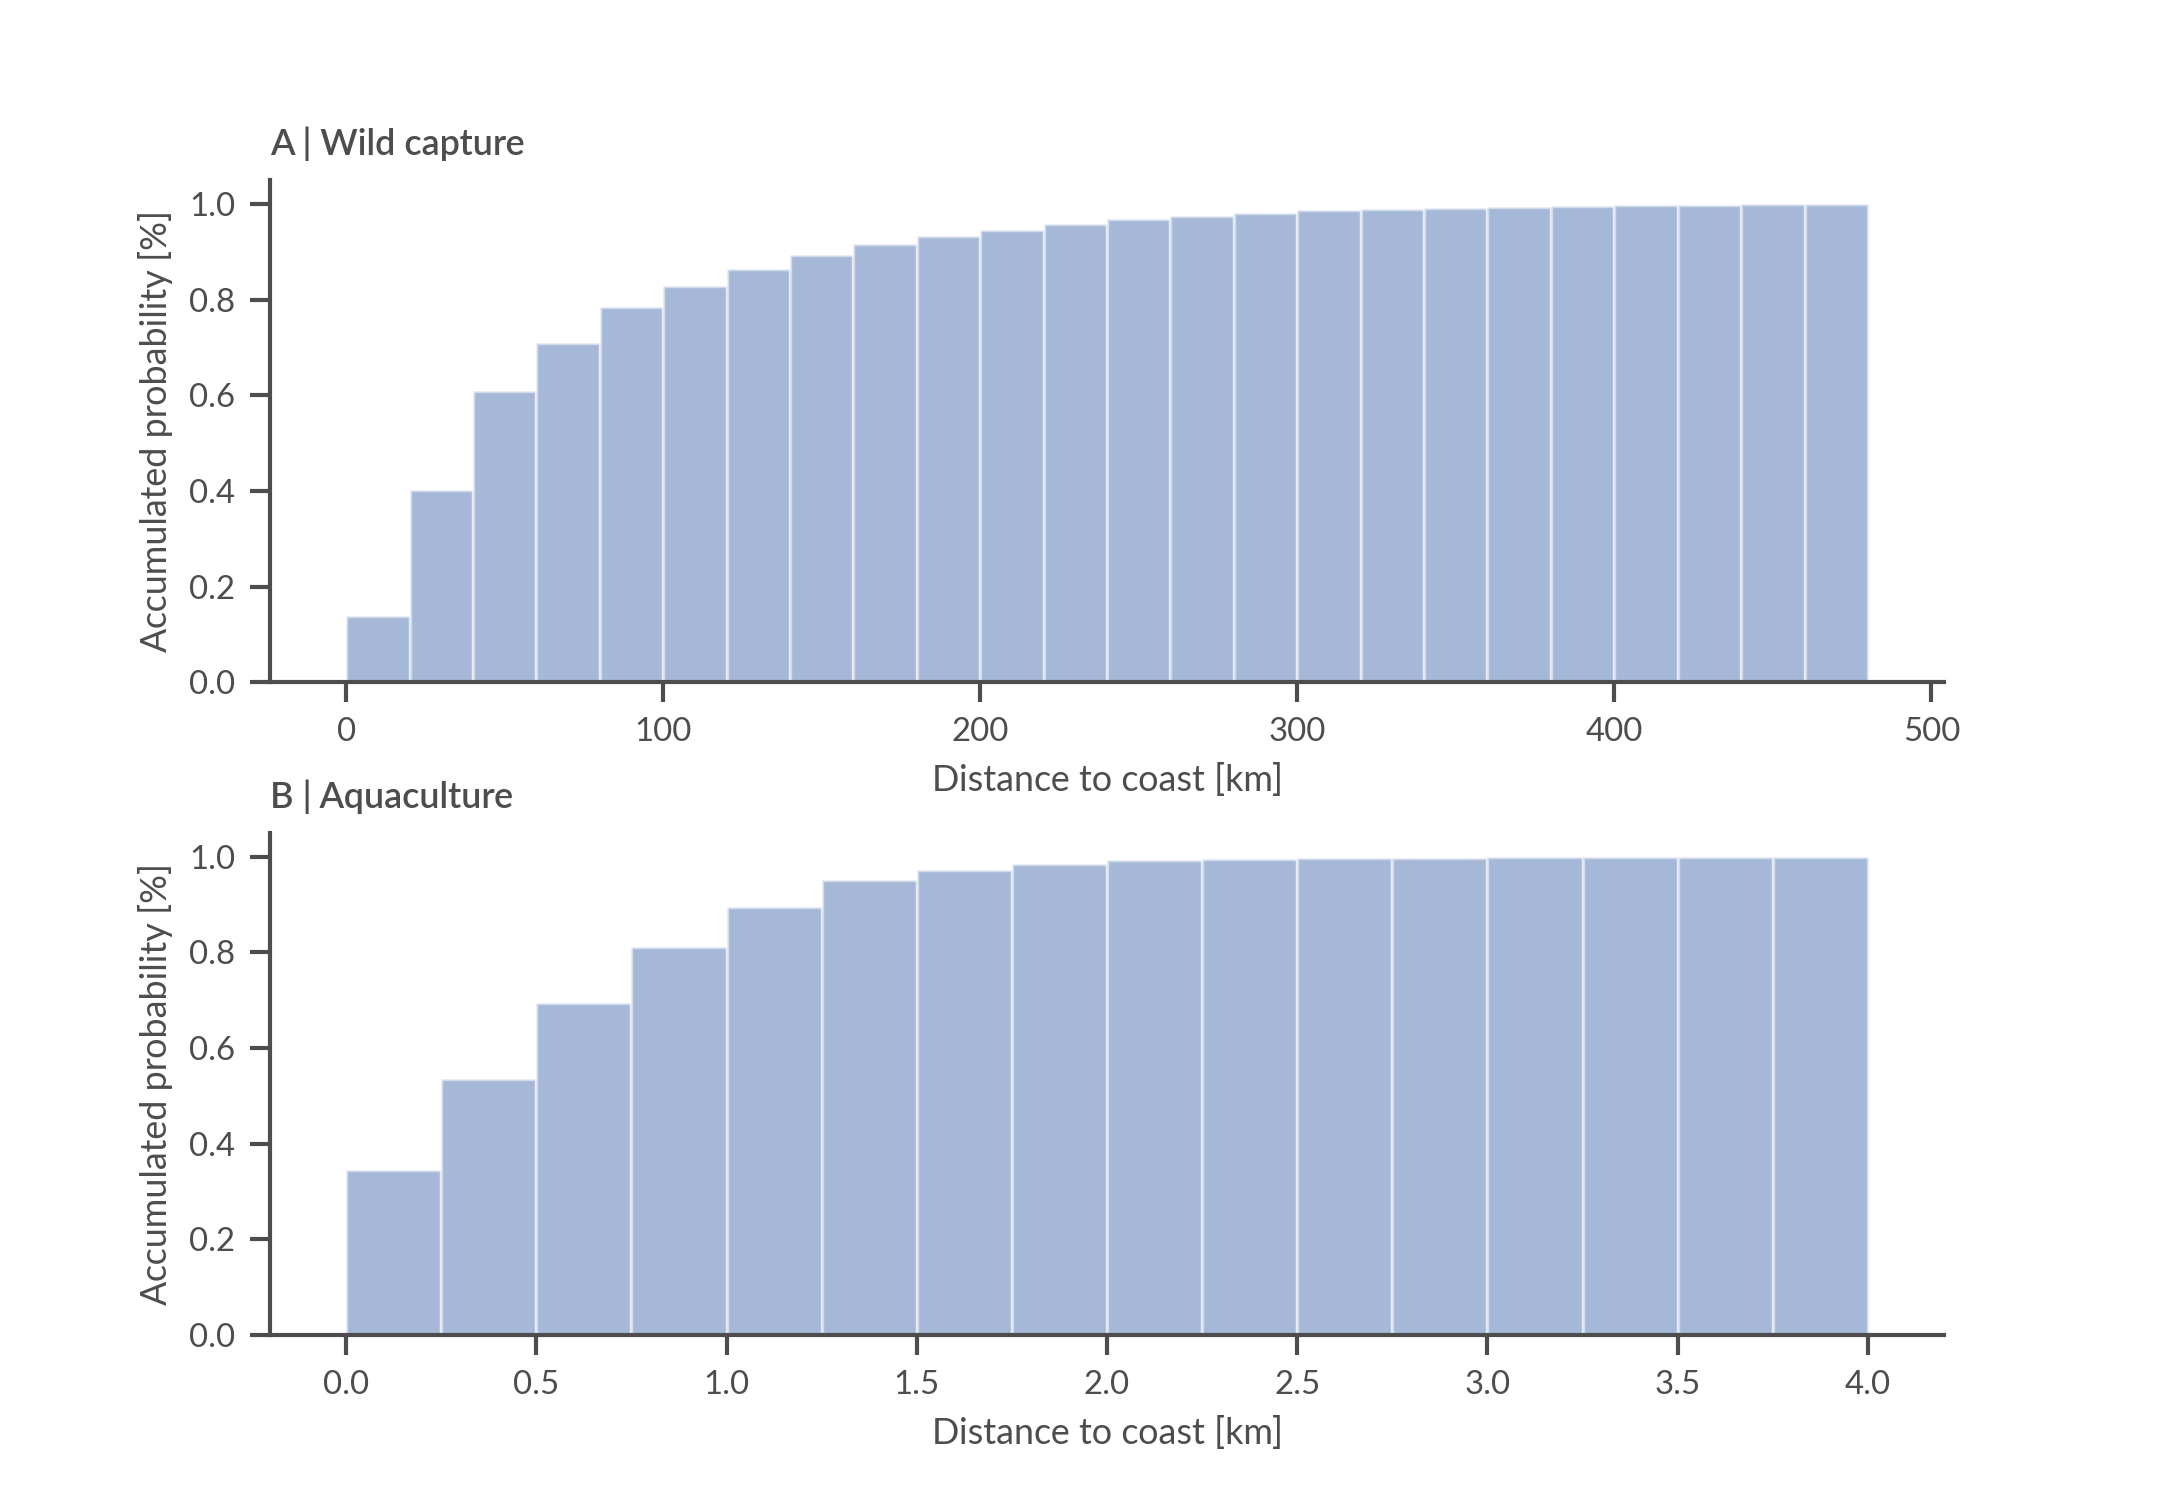
\includegraphics[width=0.95\textwidth]{fishing_aquaculture_intensity_near_coastline}
    \caption[TBD]{TBD. Reproduced with permission from Springer Nature.}
    \label{fig:TBD}
\end{figure}


\begin{figure}
    \centering
    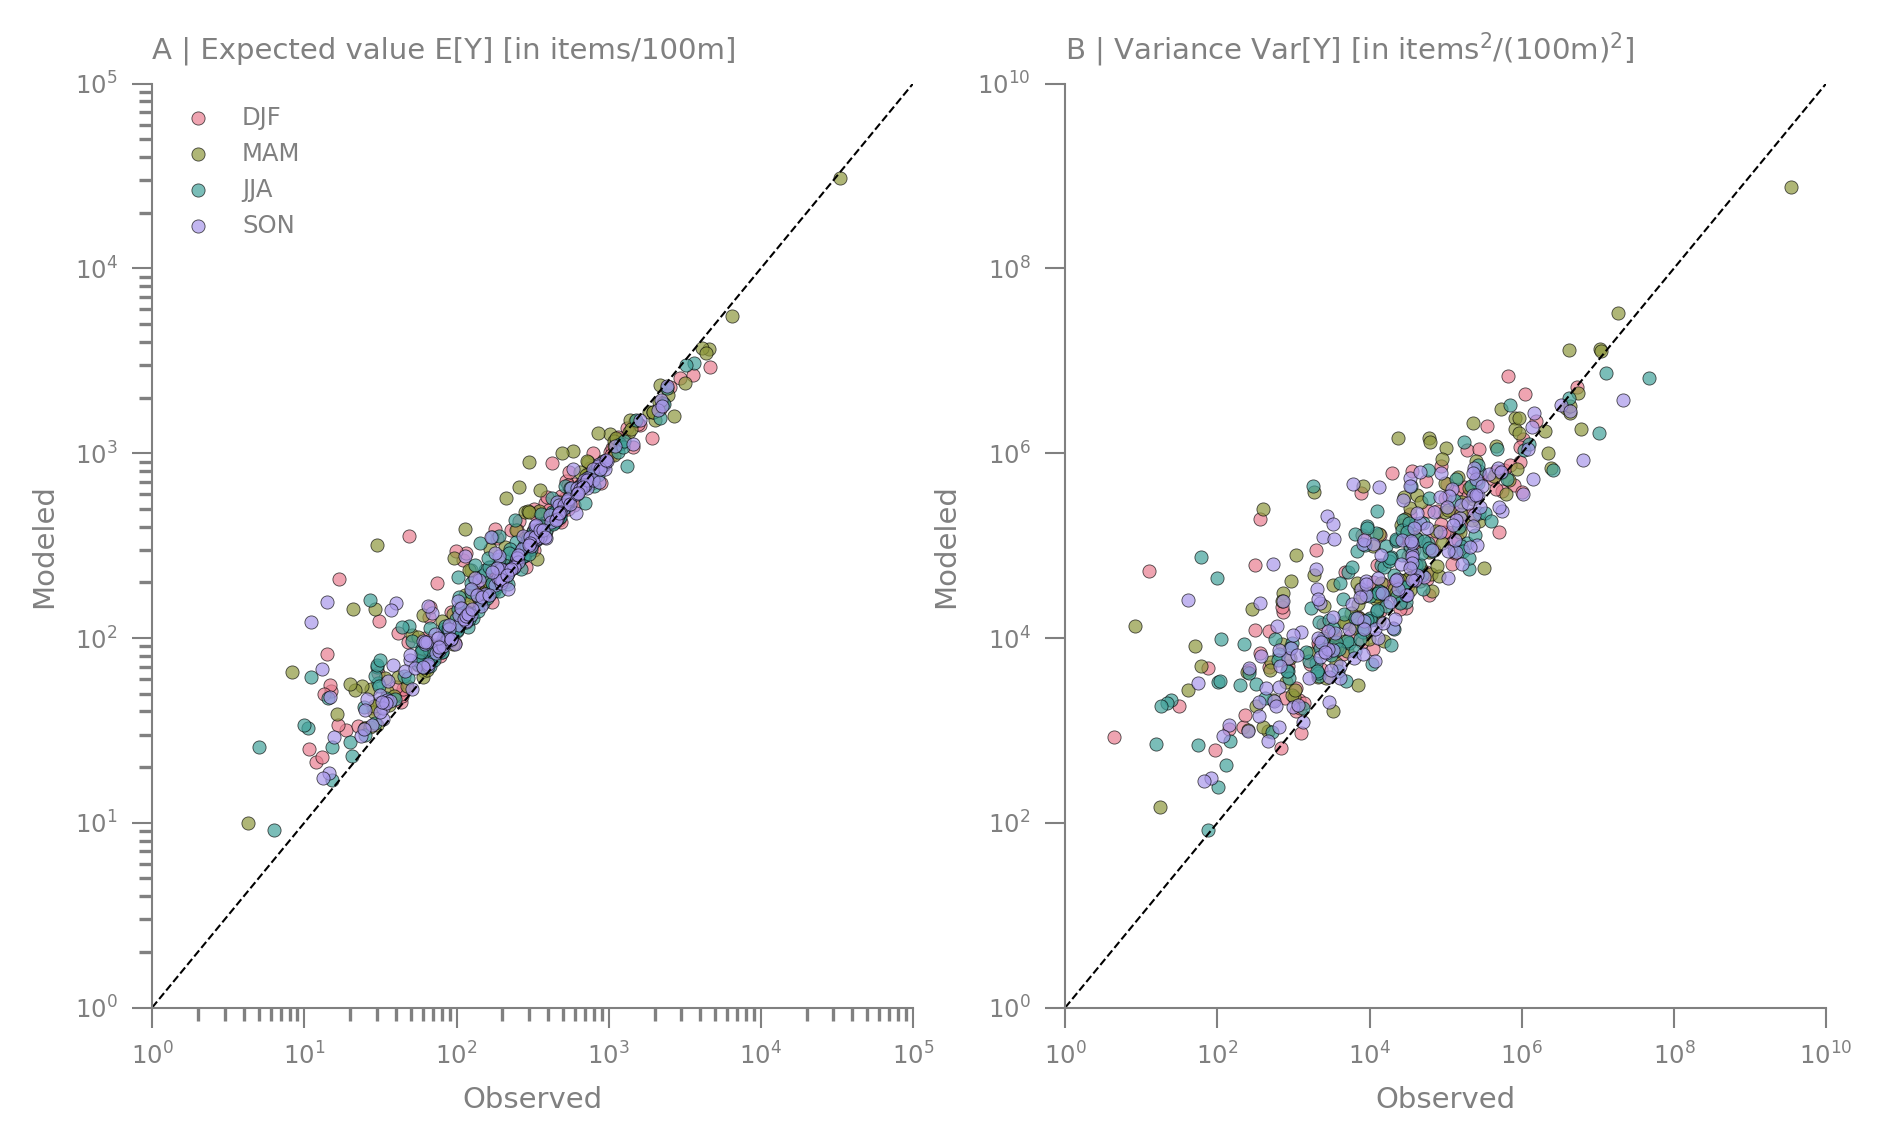
\includegraphics[width=0.95\textwidth]{lgcp_model_evaluation}
    \caption[TBD]{TBD. Reproduced with permission from Springer Nature.}
    \label{fig:TBD}
\end{figure}

\begin{figure}
    \centering
    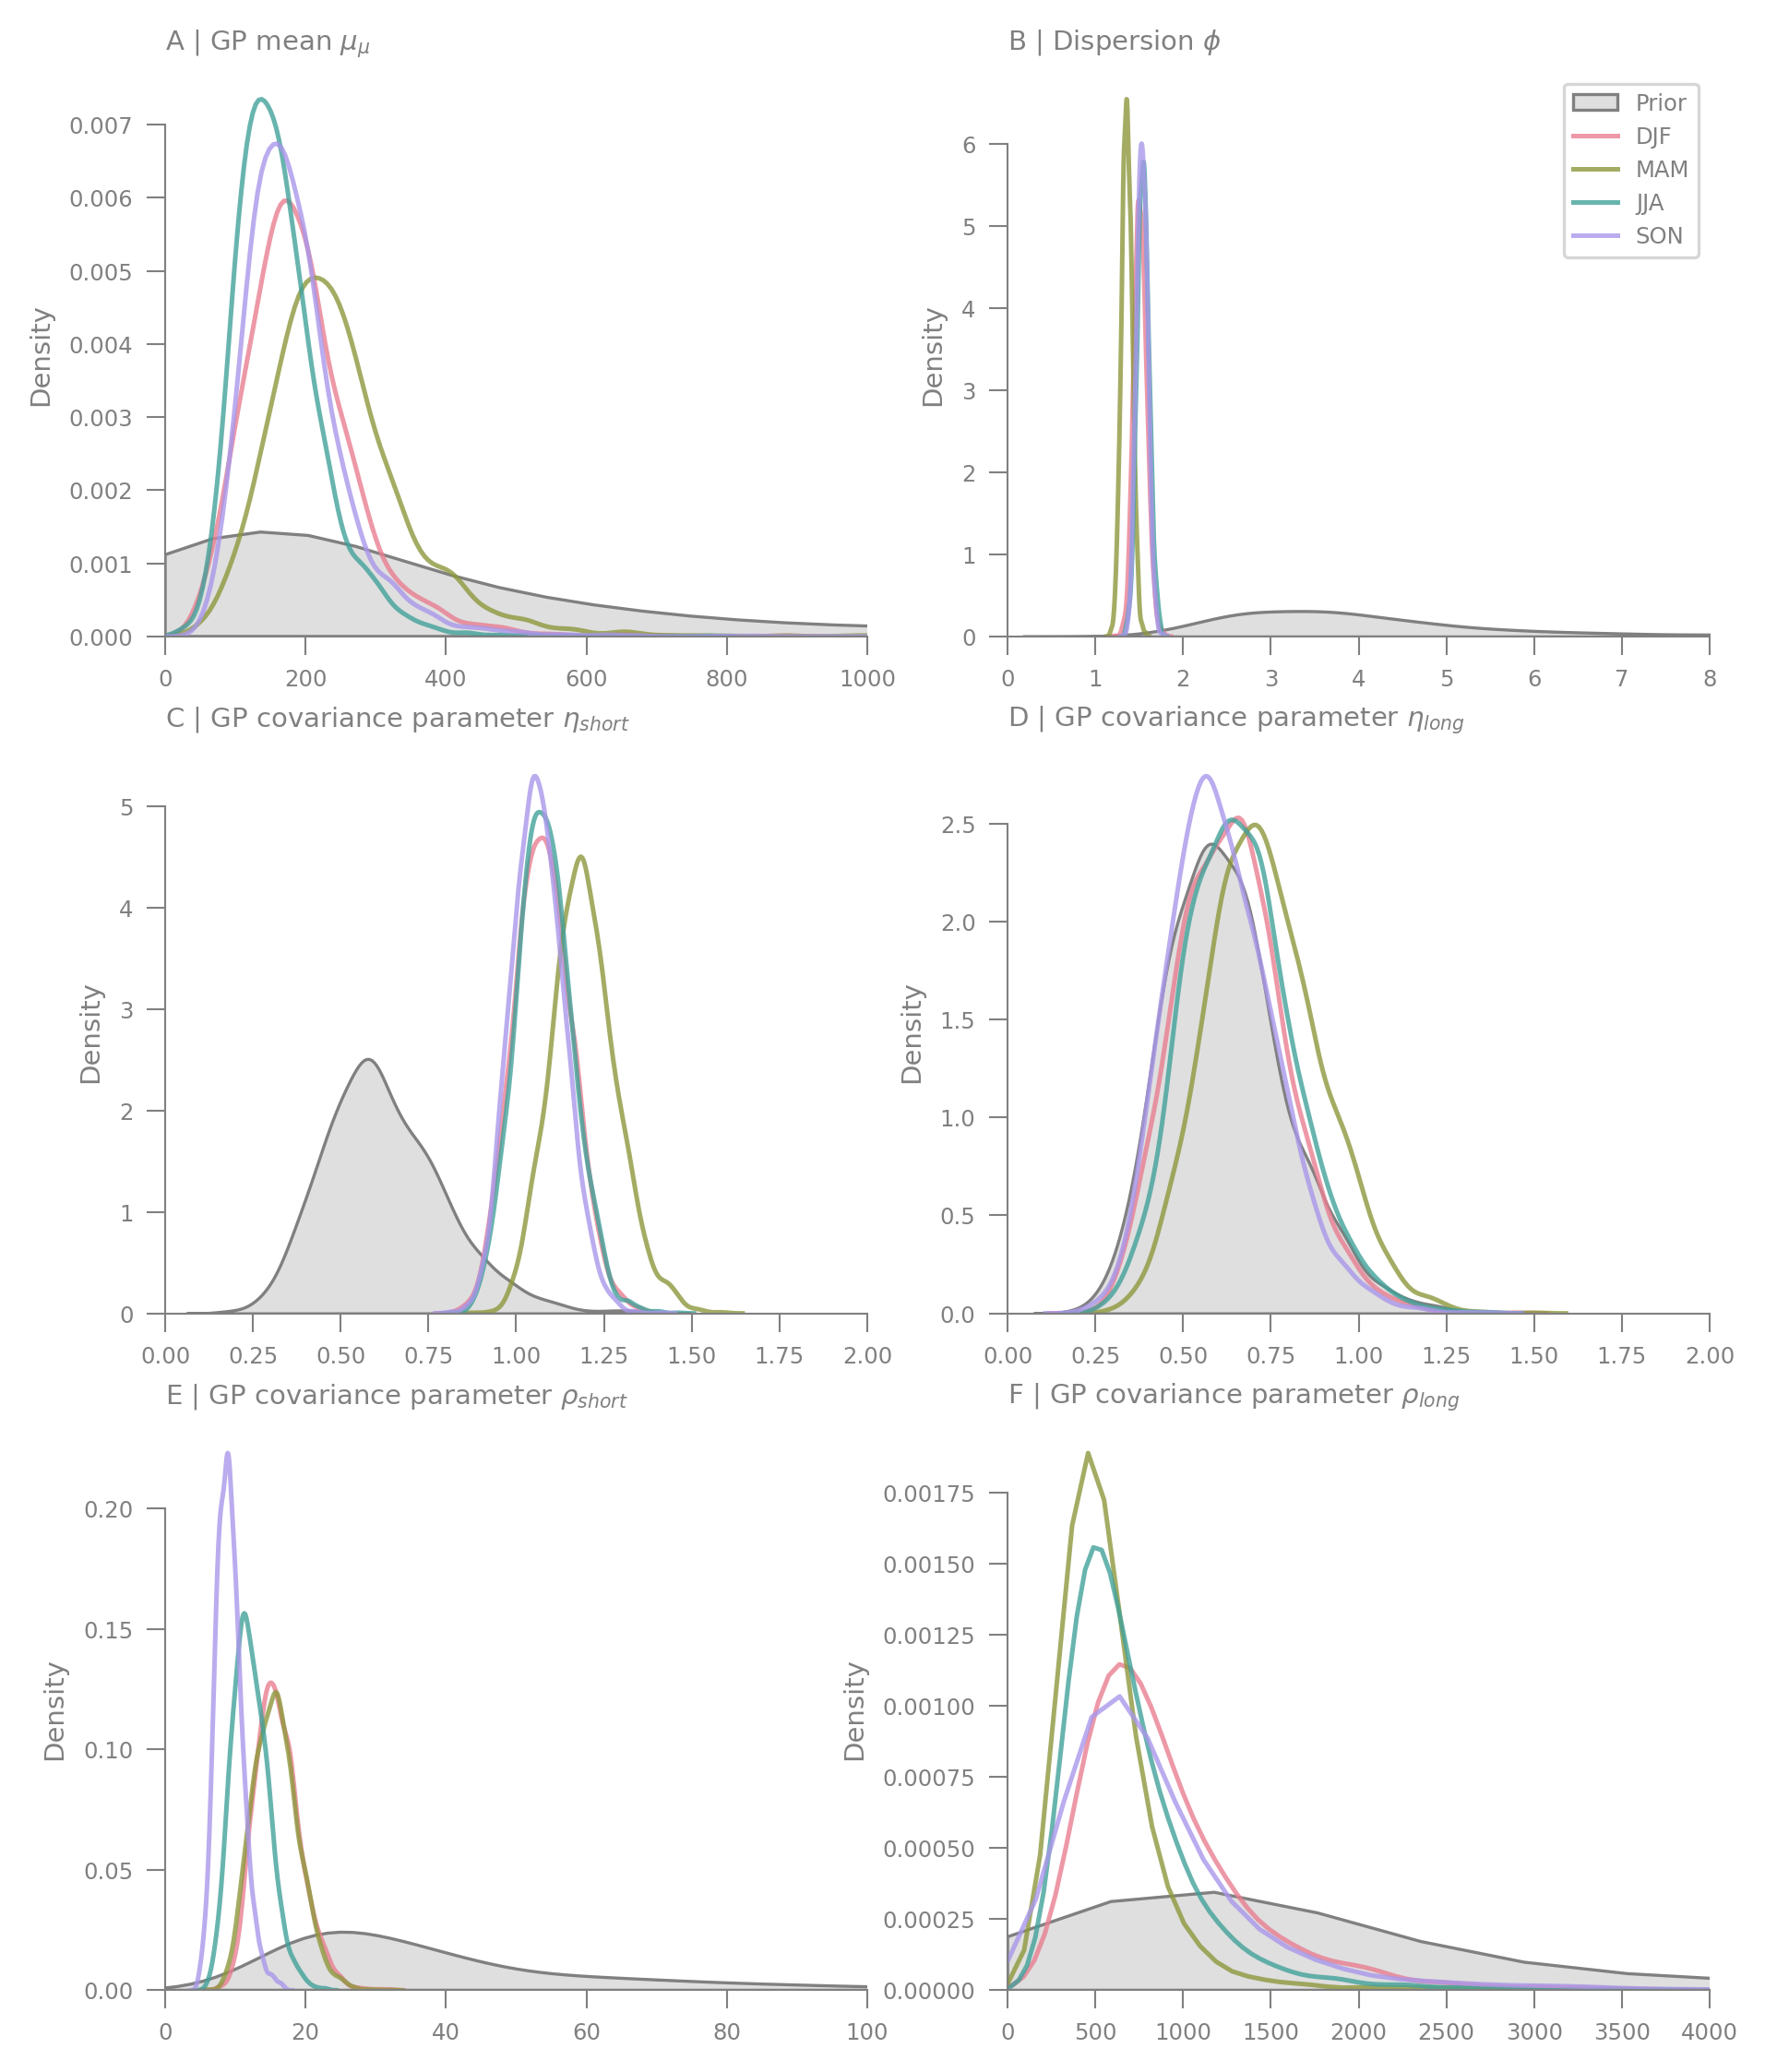
\includegraphics[width=0.95\textwidth]{lgcp_model_trace_plots}
    \caption[TBD]{TBD. Reproduced with permission from Springer Nature.}
    \label{fig:TBD}
\end{figure}

\begin{figure}
    \centering
    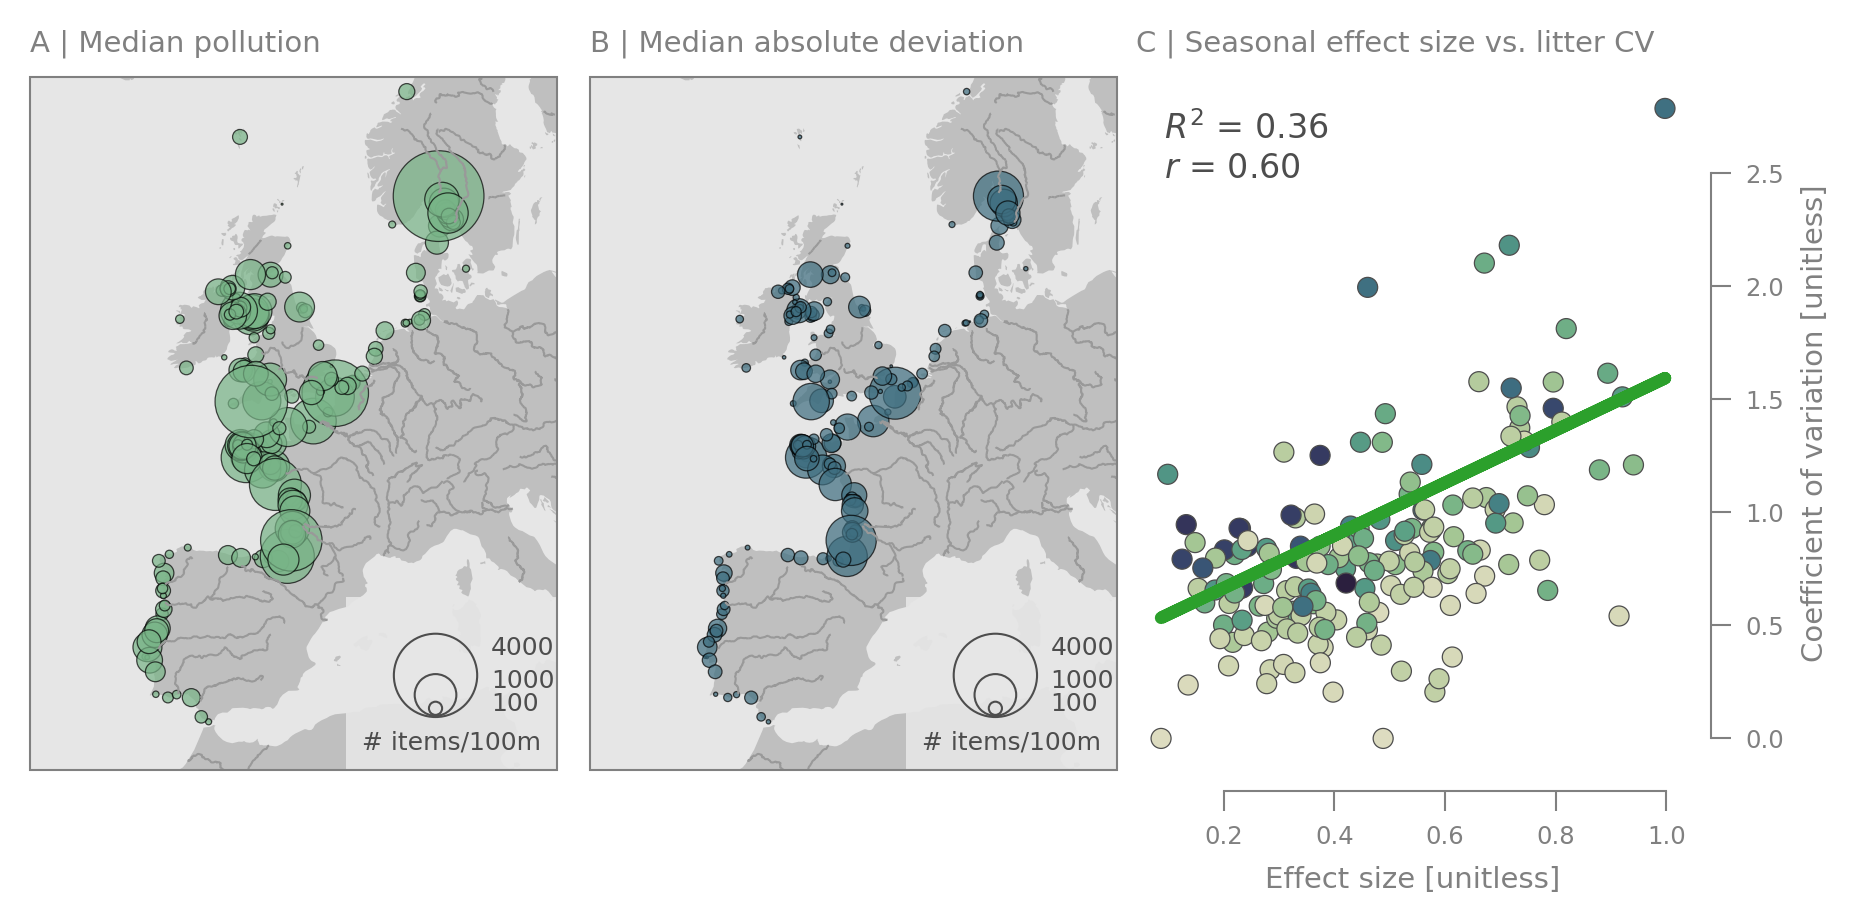
\includegraphics[width=0.95\textwidth]{ospar_variance_seasonality}
    \caption[TBD]{TBD. Reproduced with permission from Springer Nature.}
    \label{fig:TBD}
\end{figure}

\begin{figure}
    \centering
    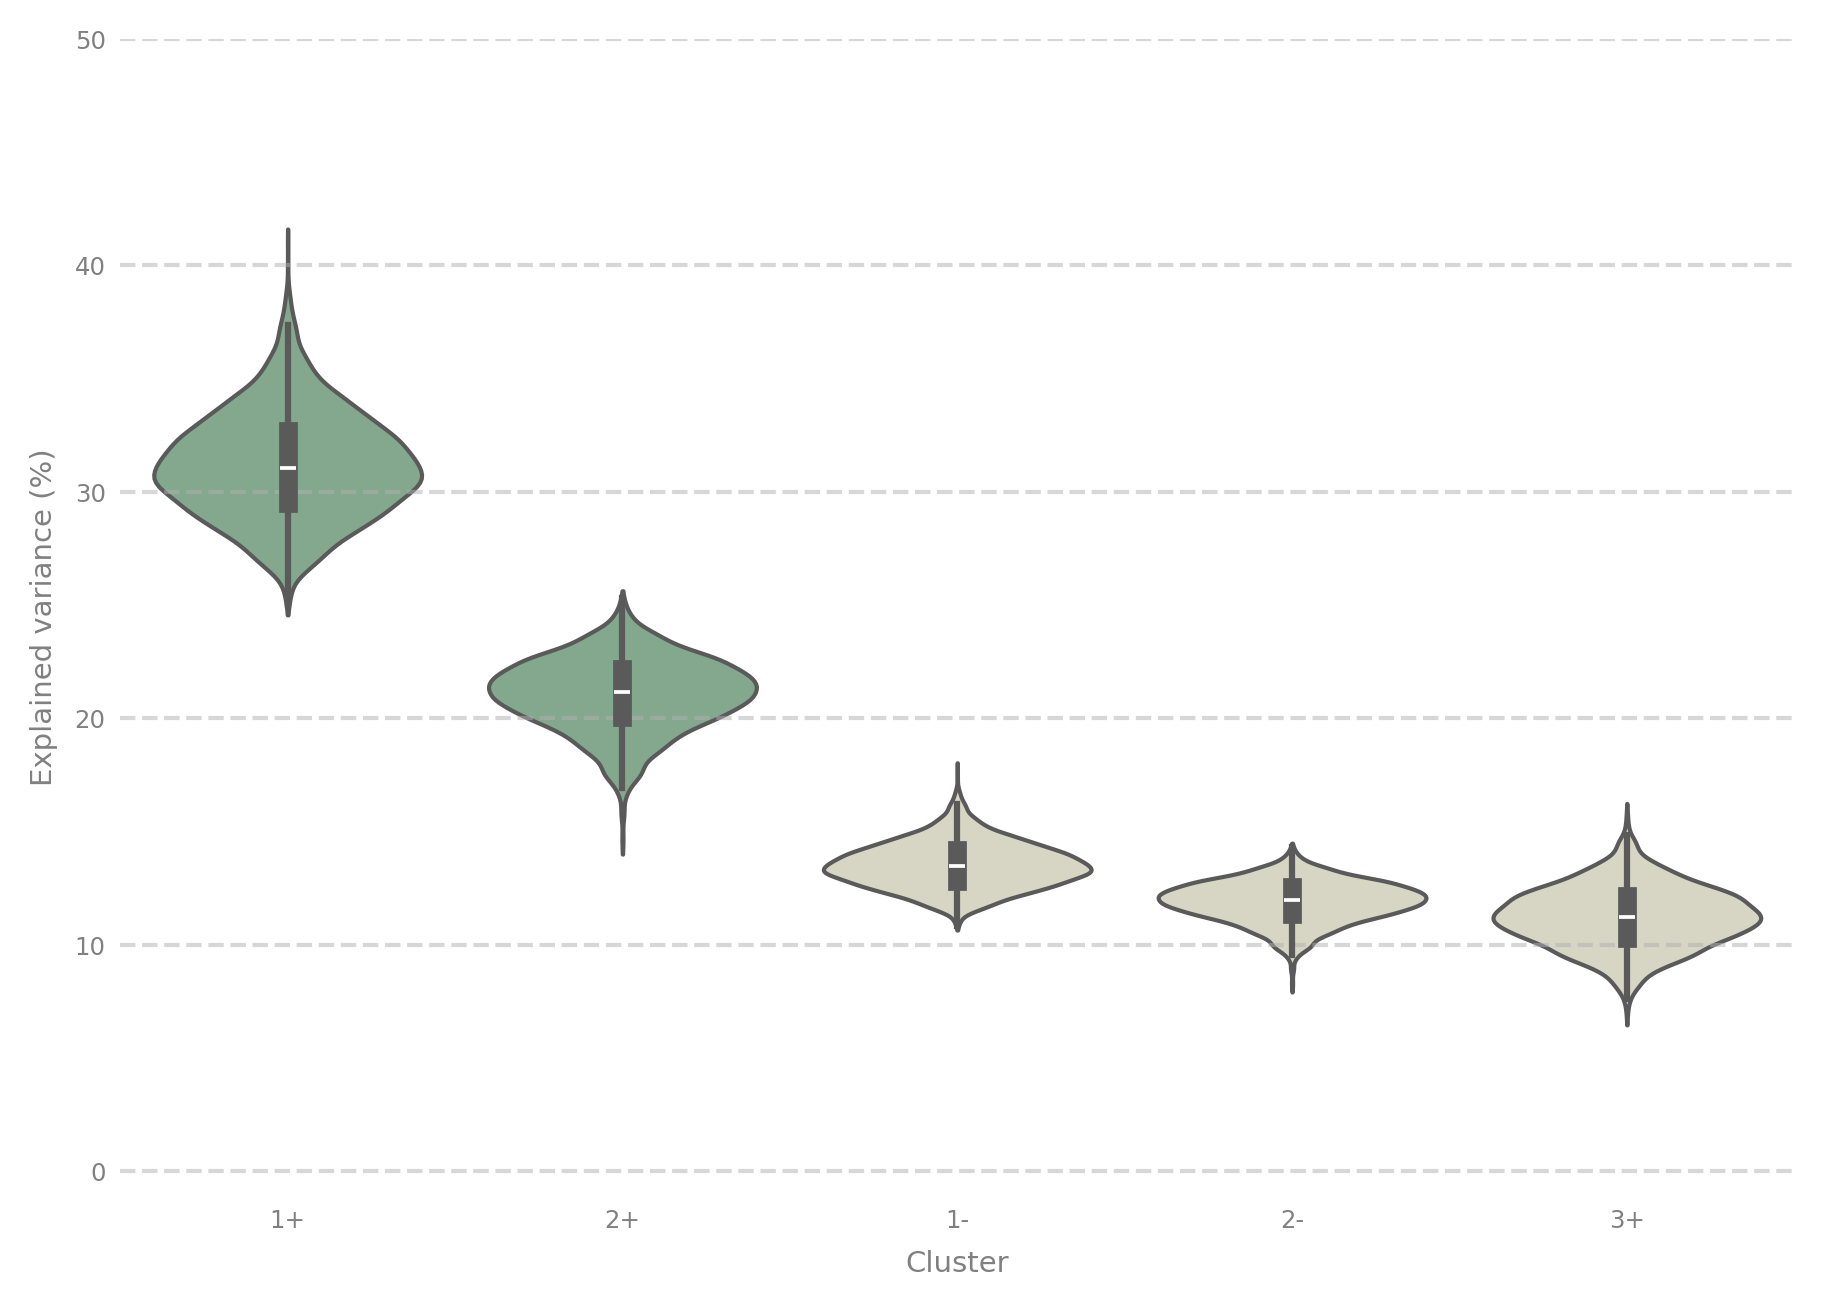
\includegraphics[width=0.95\textwidth]{plastic_clustering_explained_variance}
    \caption[TBD]{TBD. Reproduced with permission from Springer Nature.}
    \label{fig:TBD}
\end{figure}

\begin{figure}
    \centering
    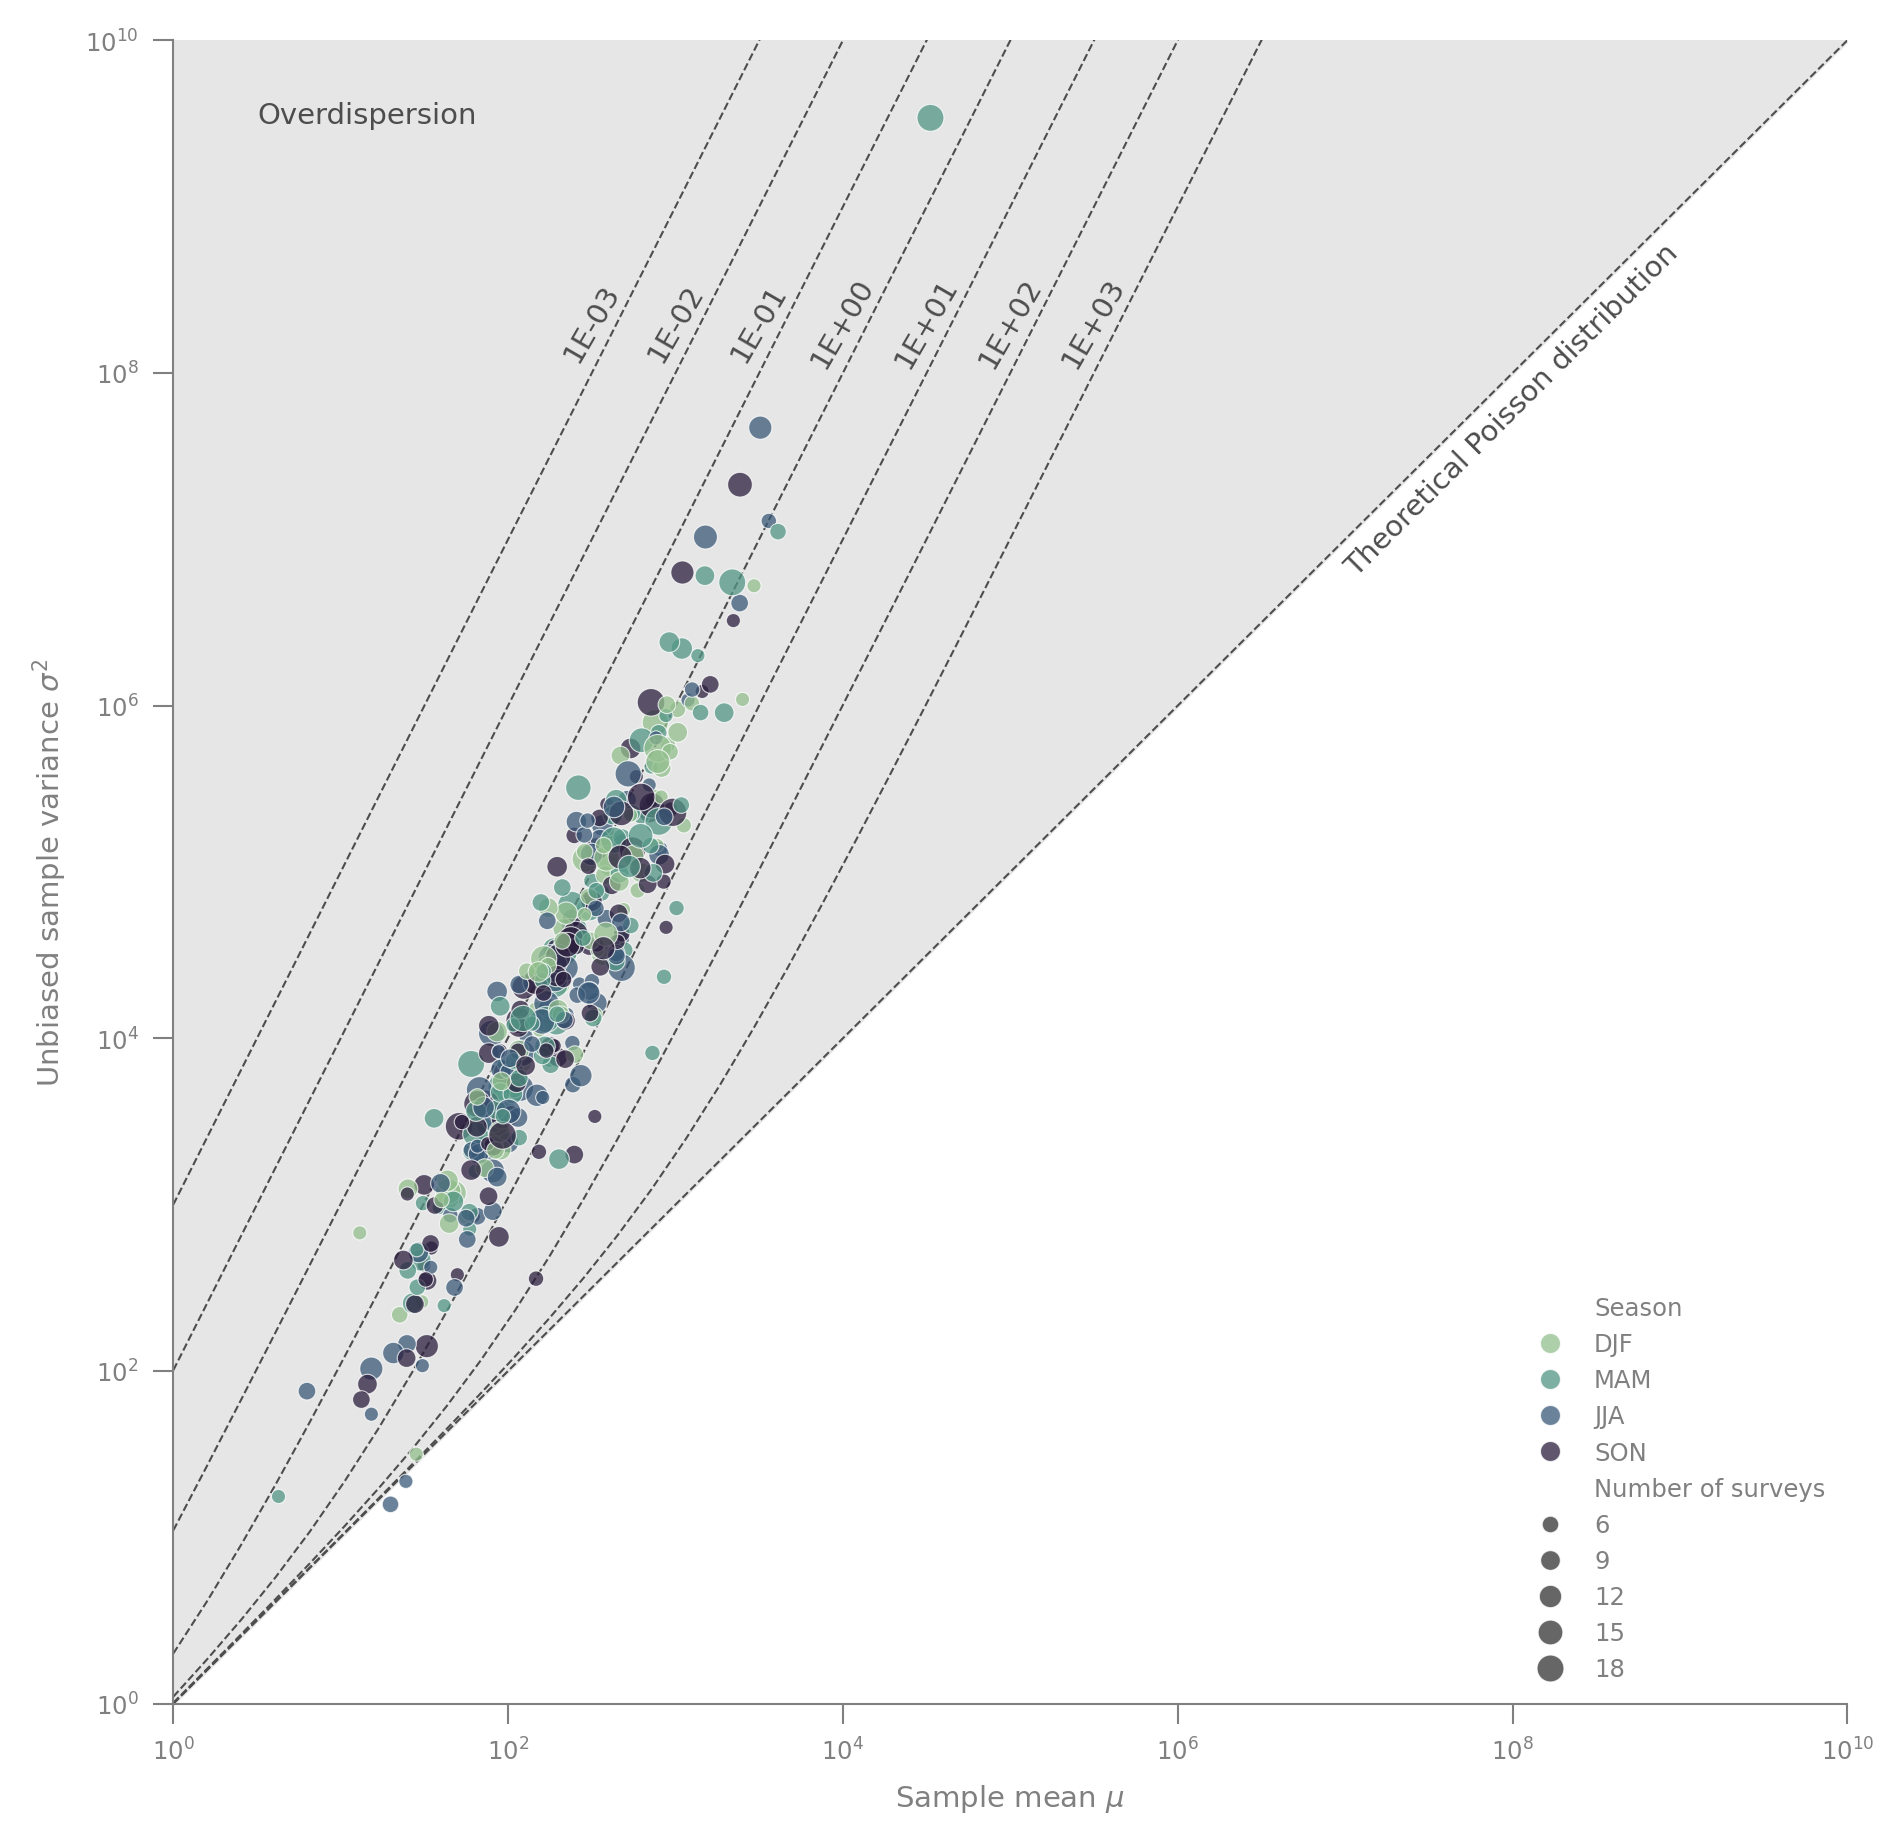
\includegraphics[width=0.95\textwidth]{plastic_overdispersion}
    \caption[TBD]{TBD. Reproduced with permission from Springer Nature.}
    \label{fig:TBD}
\end{figure}

\begin{figure}
    \centering
    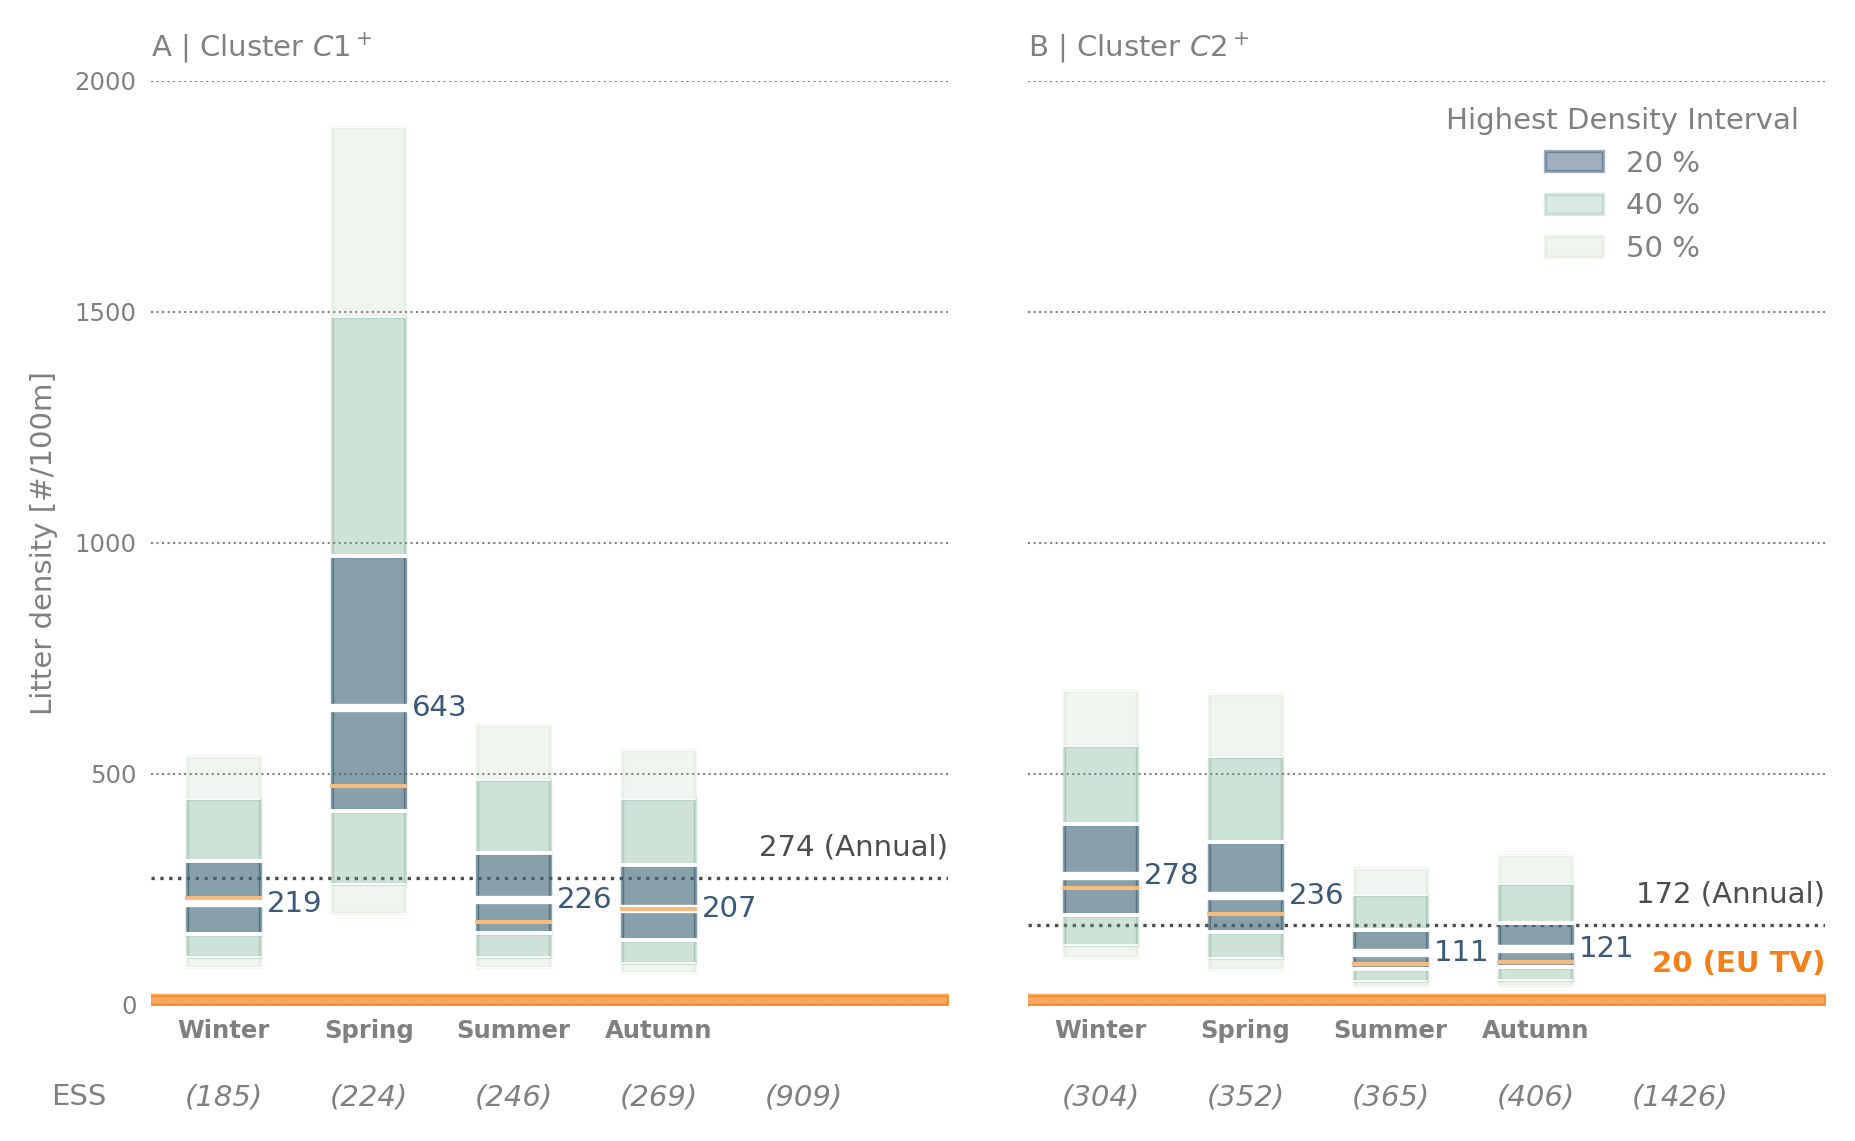
\includegraphics[width=0.95\textwidth]{plastics_clusters_boxplot}
    \caption[TBD]{TBD. Reproduced with permission from Springer Nature.}
    \label{fig:TBD}
\end{figure}

\begin{figure}
    \centering
    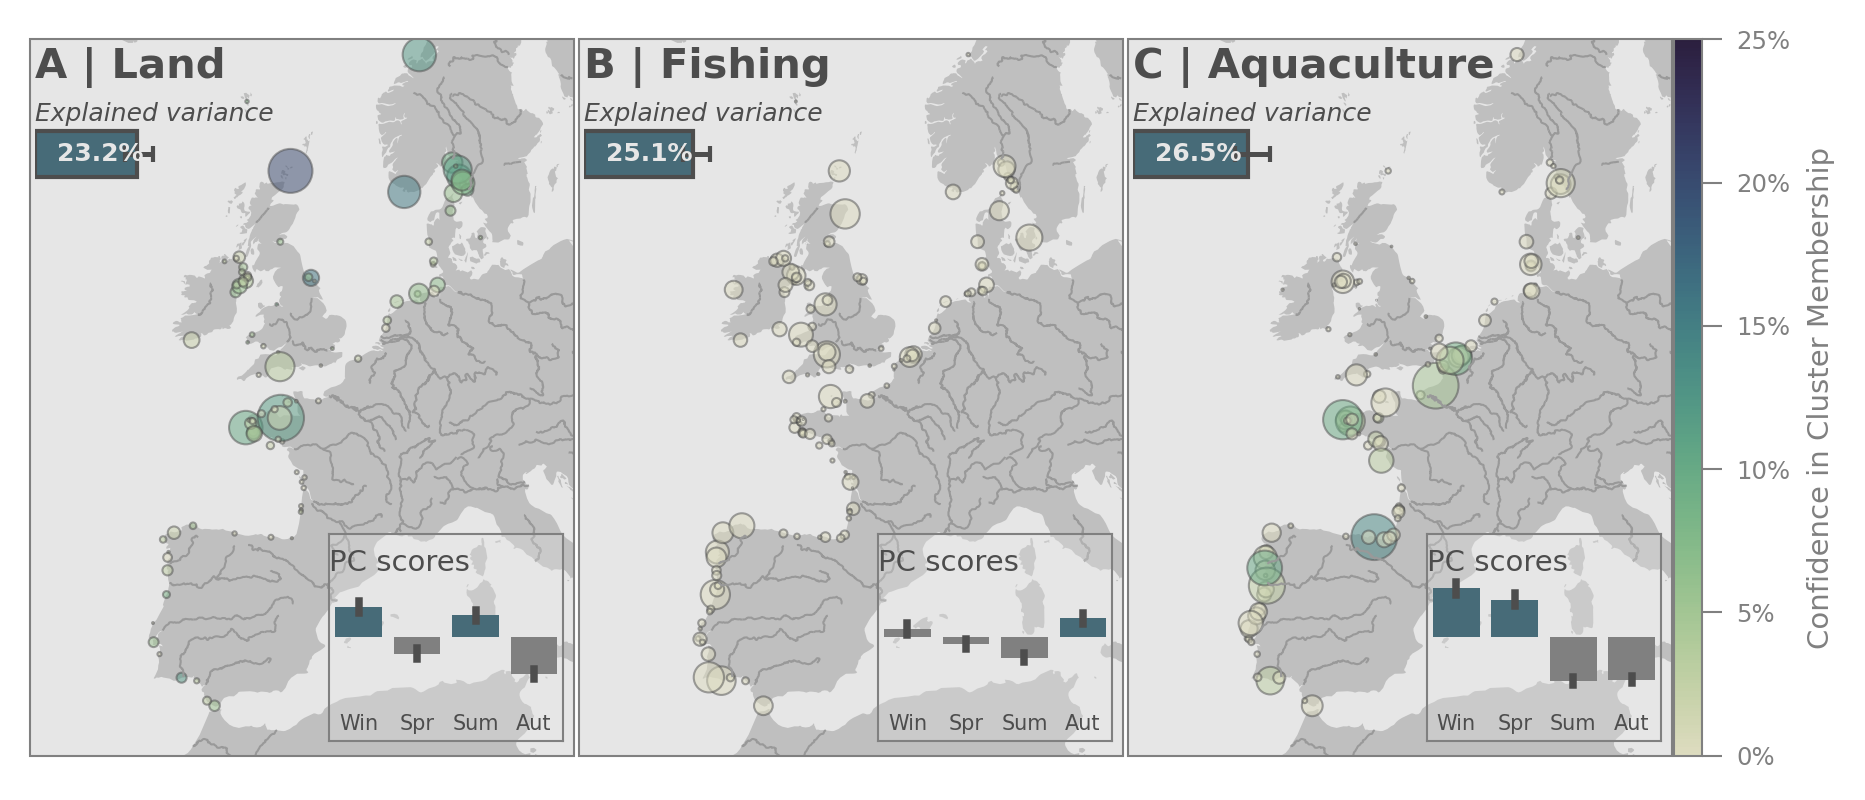
\includegraphics[width=0.95\textwidth]{plastics_clusters_fraction_map}
    \caption[TBD]{TBD. Reproduced with permission from Springer Nature.}
    \label{fig:TBD}
\end{figure}

\begin{figure}
    \centering
    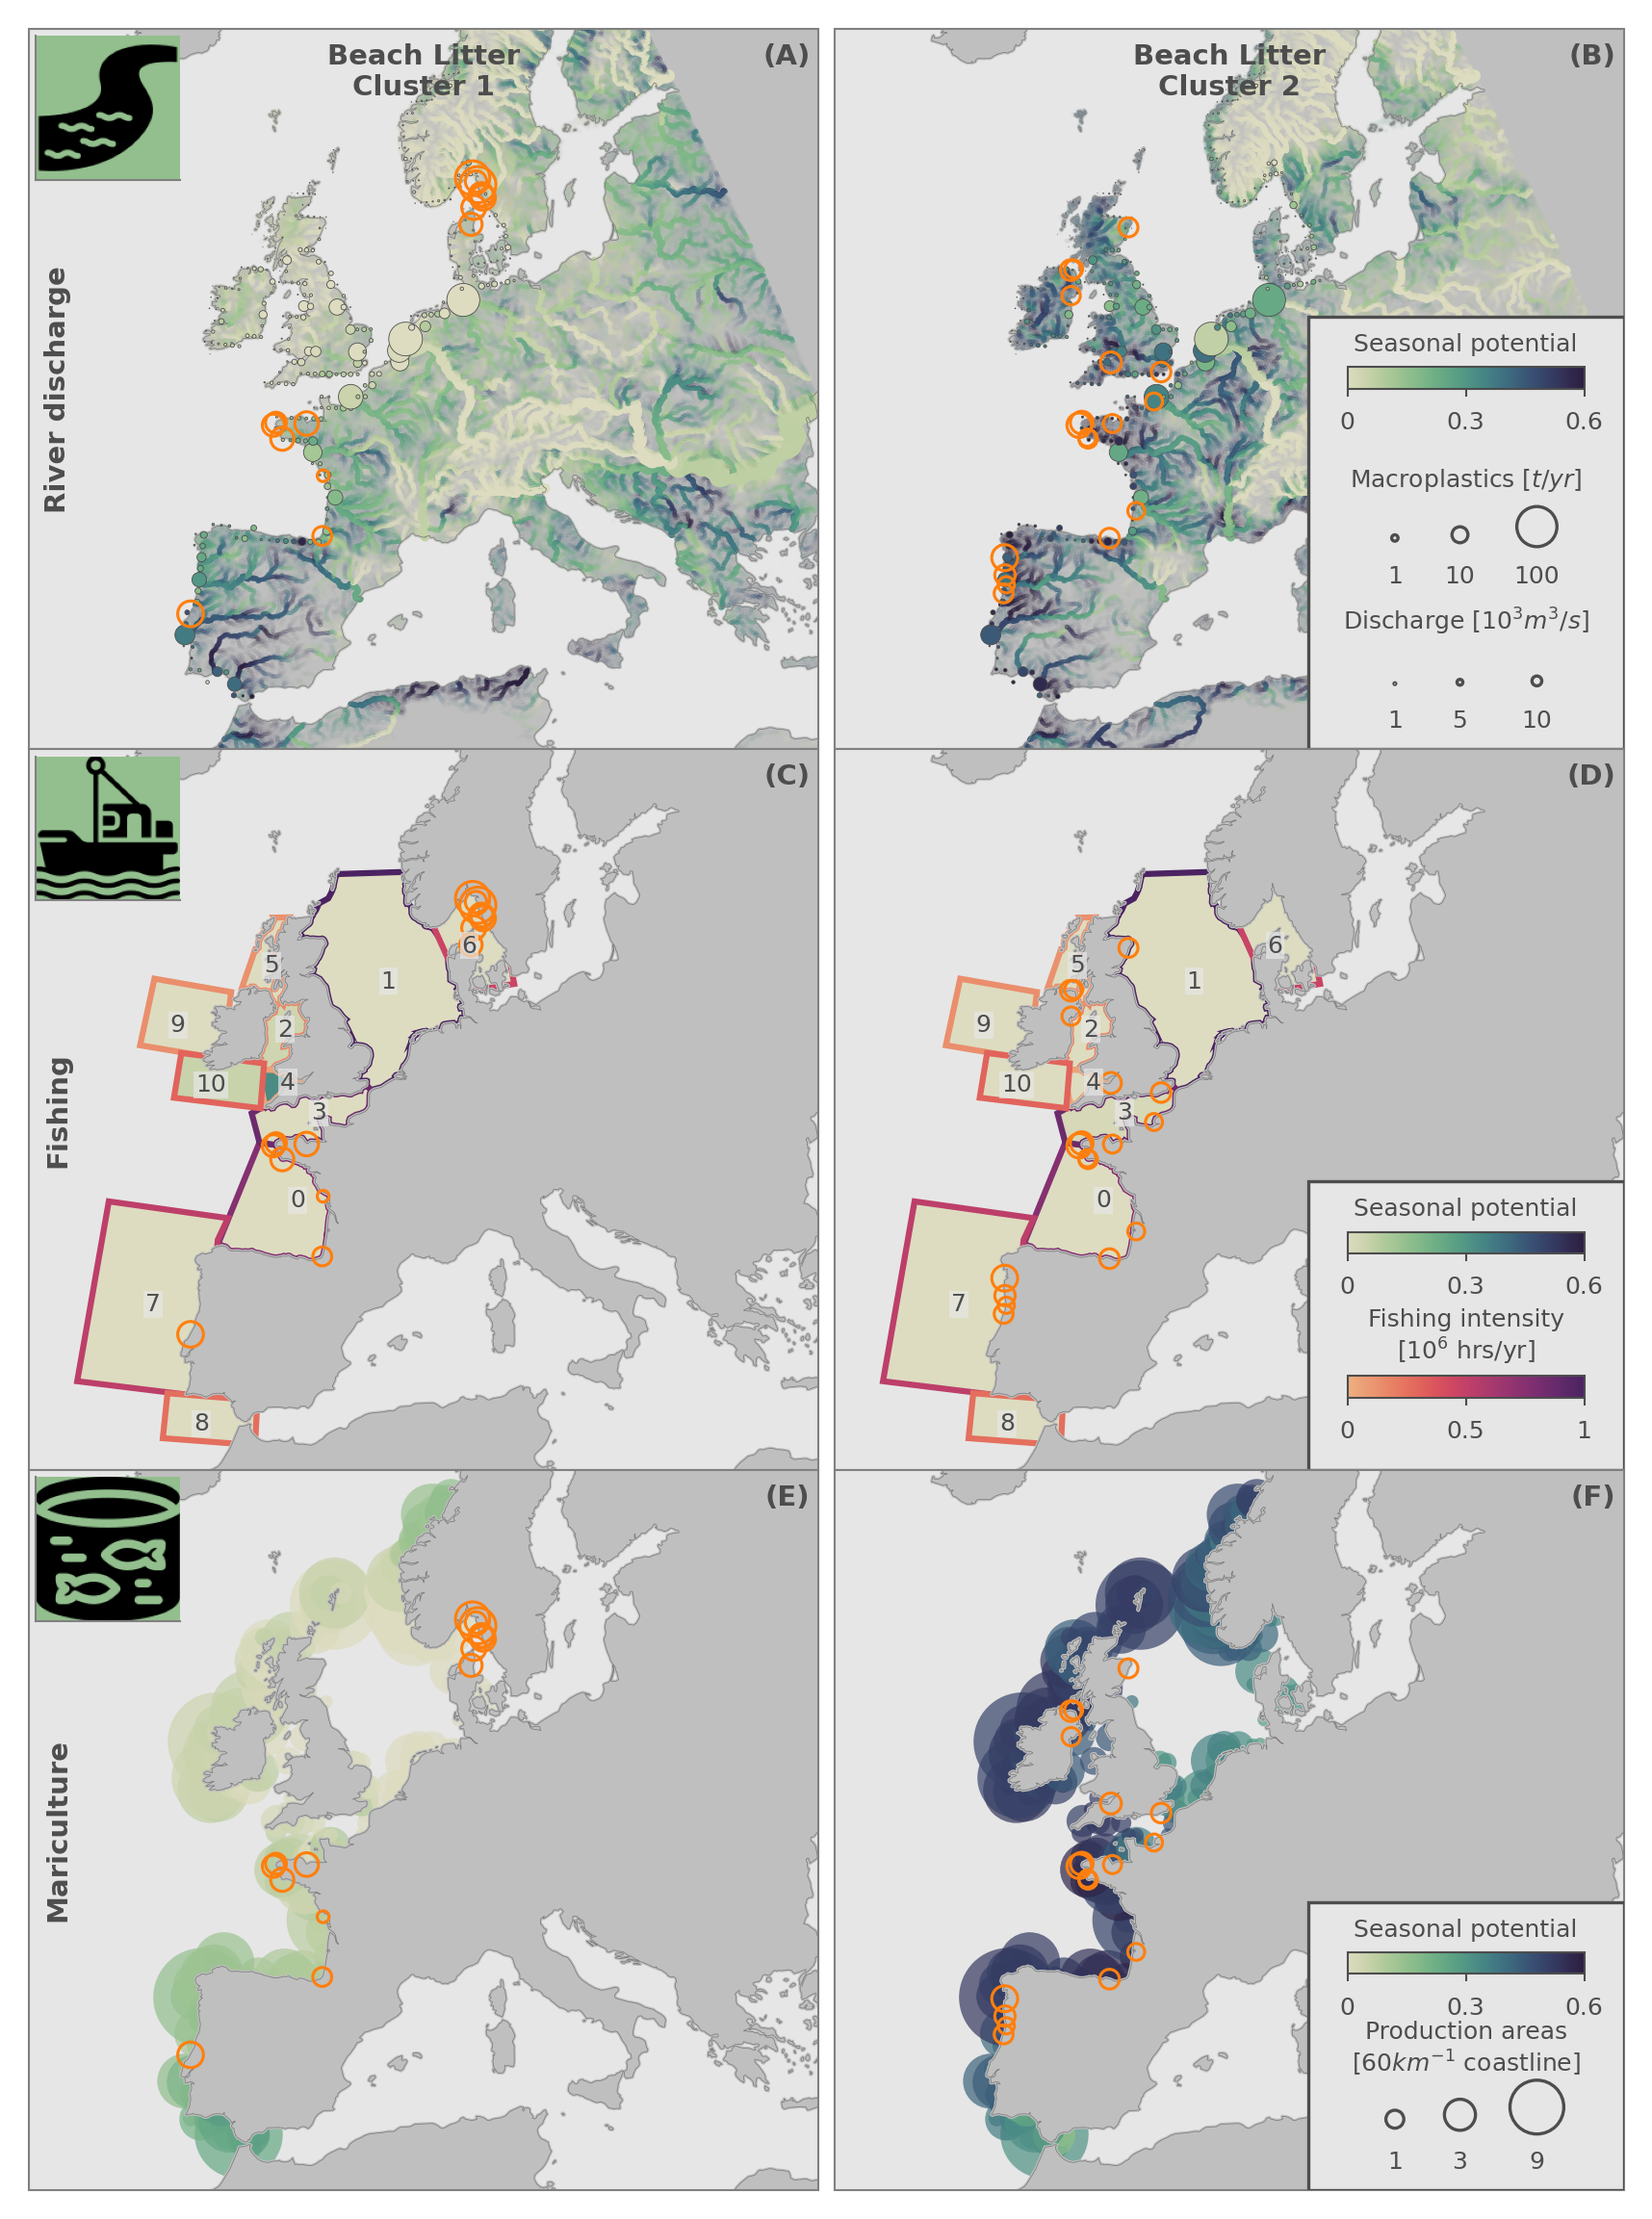
\includegraphics[width=0.95\textwidth]{plastics_seasonal_potential}
    \caption[TBD]{TBD. Reproduced with permission from Springer Nature.}
    \label{fig:TBD}
\end{figure}

\begin{figure}
    \centering
    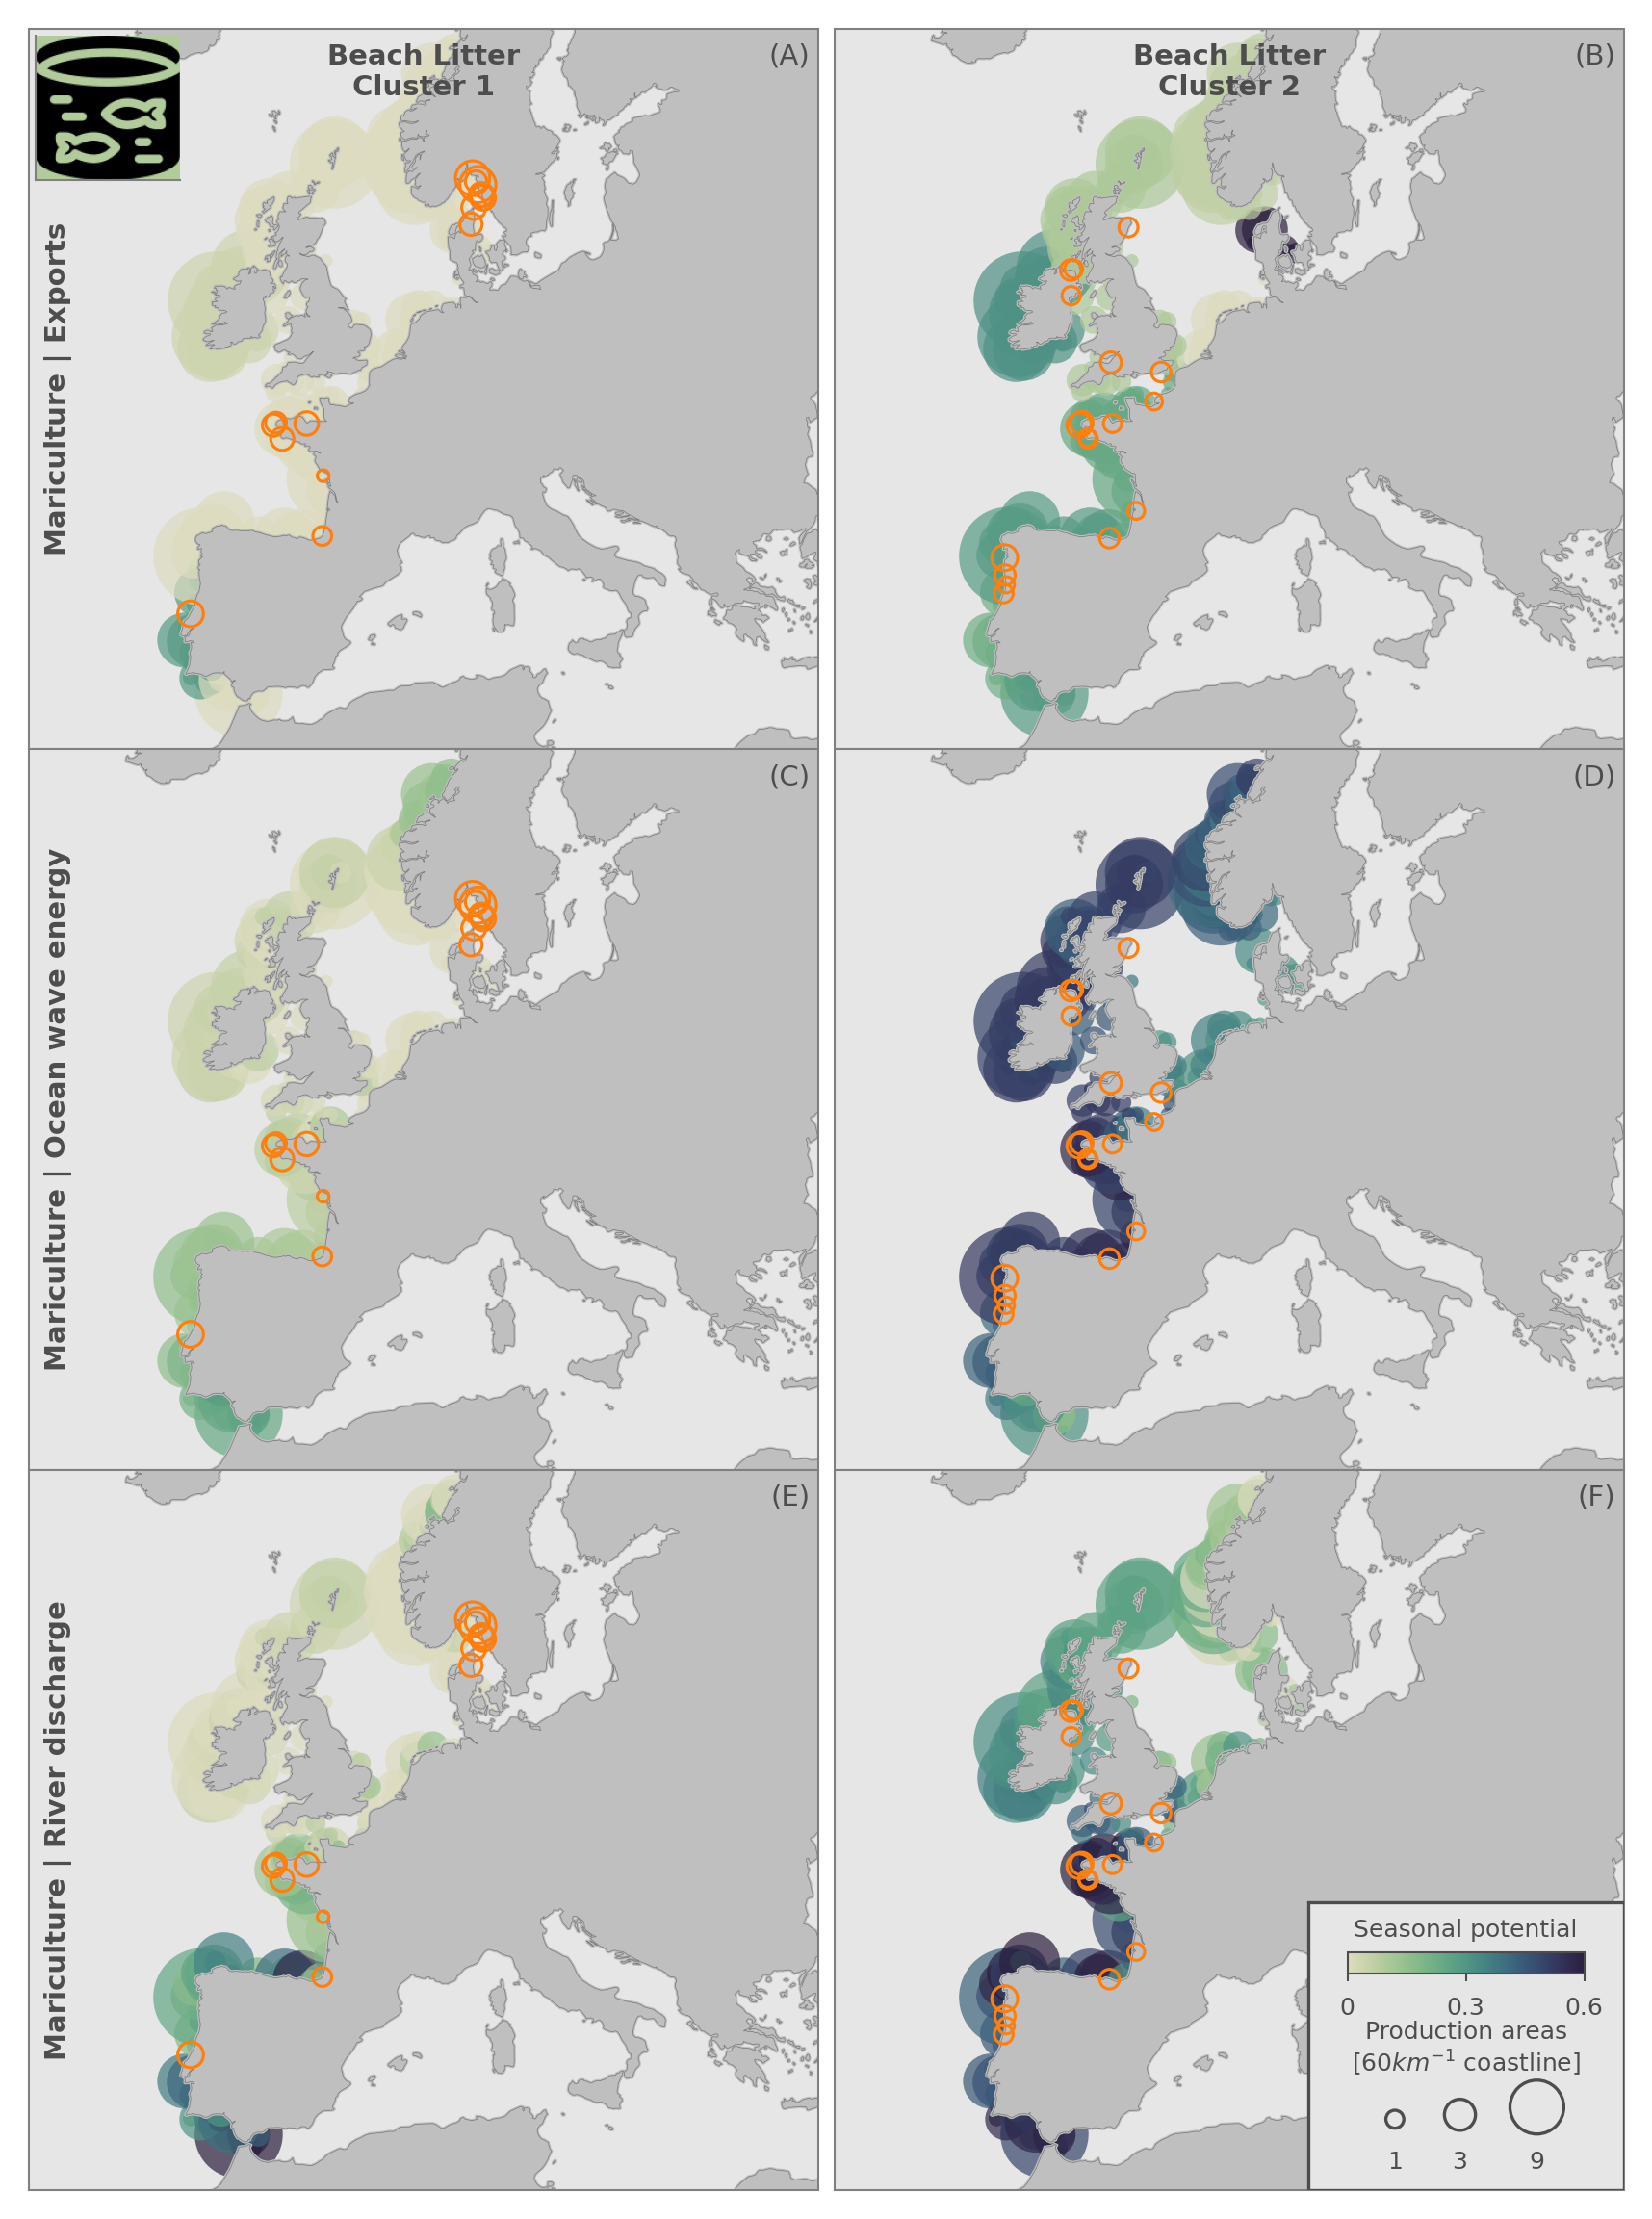
\includegraphics[width=0.95\textwidth]{plastics_seasonal_potential_mariculture}
    \caption[TBD]{TBD. Reproduced with permission from Springer Nature.}
    \label{fig:TBD}
\end{figure}

\begin{figure}
    \centering
    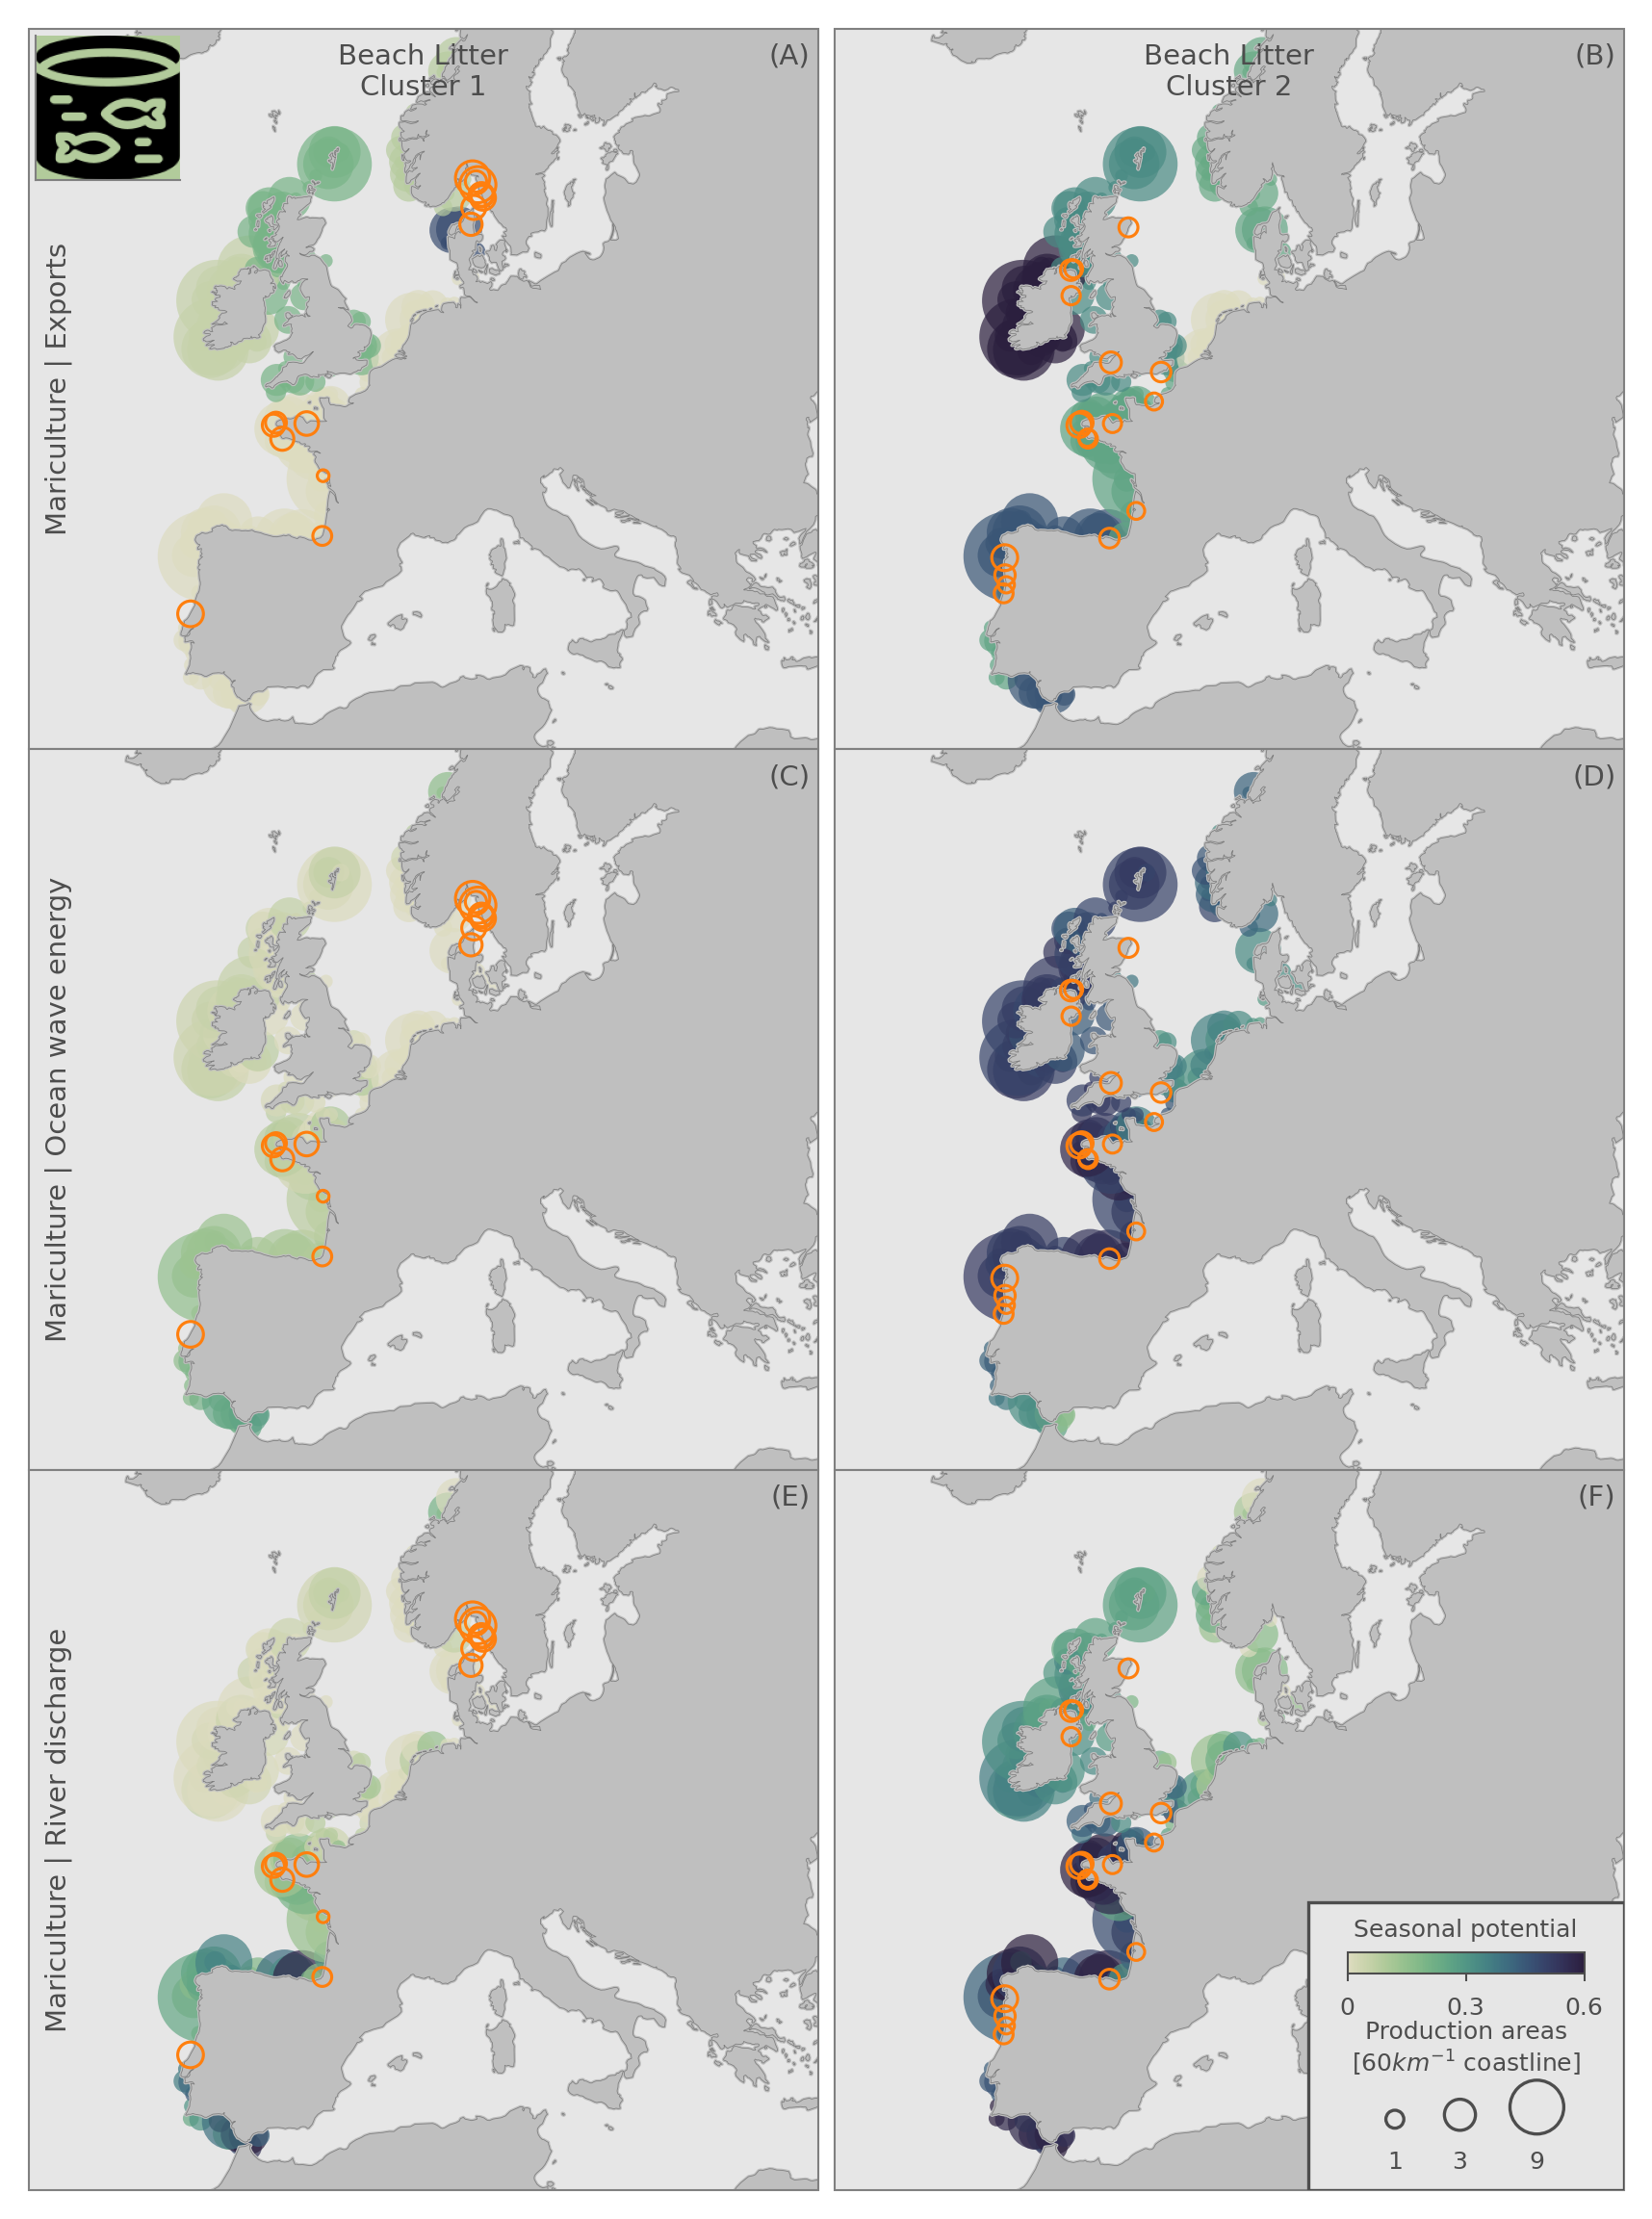
\includegraphics[width=0.95\textwidth]{plastics_seasonal_potential_mariculture_bivalve}
    \caption[TBD]{TBD. Reproduced with permission from Springer Nature.}
    \label{fig:TBD}
\end{figure}

\begin{figure}
    \centering
    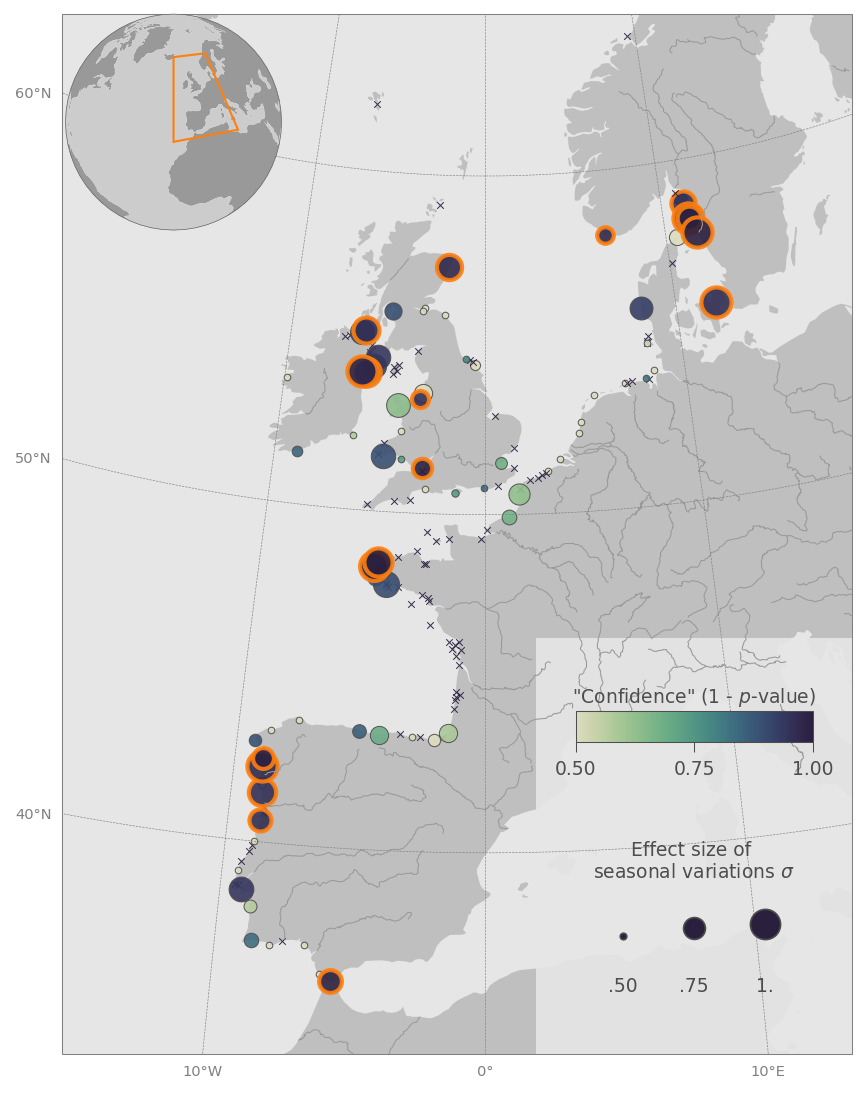
\includegraphics[width=0.95\textwidth]{plastics_seasonality_map_isolated}
    \caption[TBD]{TBD. Reproduced with permission from Springer Nature.}
    \label{fig:TBD}
\end{figure}

\begin{figure}
    \centering
    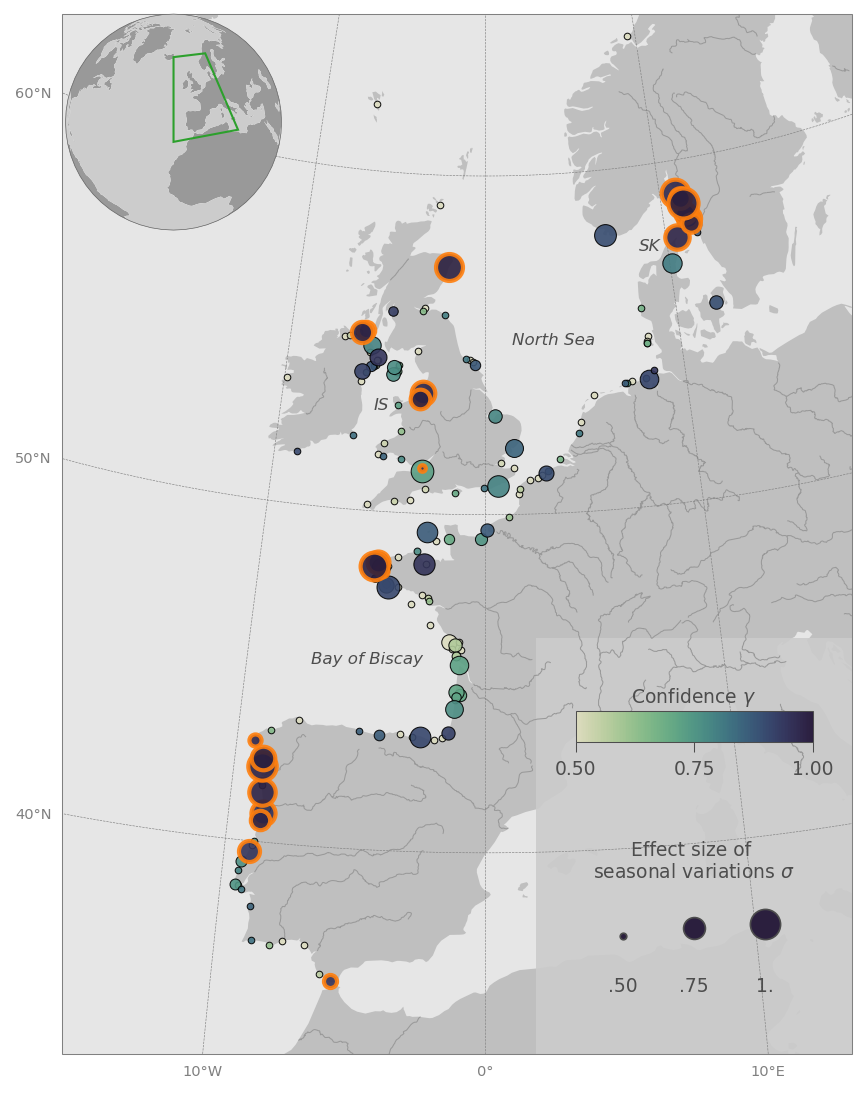
\includegraphics[width=0.95\textwidth]{plastics_seasonality_map_lgcp}
    \caption[TBD]{TBD. Reproduced with permission from Springer Nature.}
    \label{fig:TBD}
\end{figure}


\begin{figure}
    \centering
    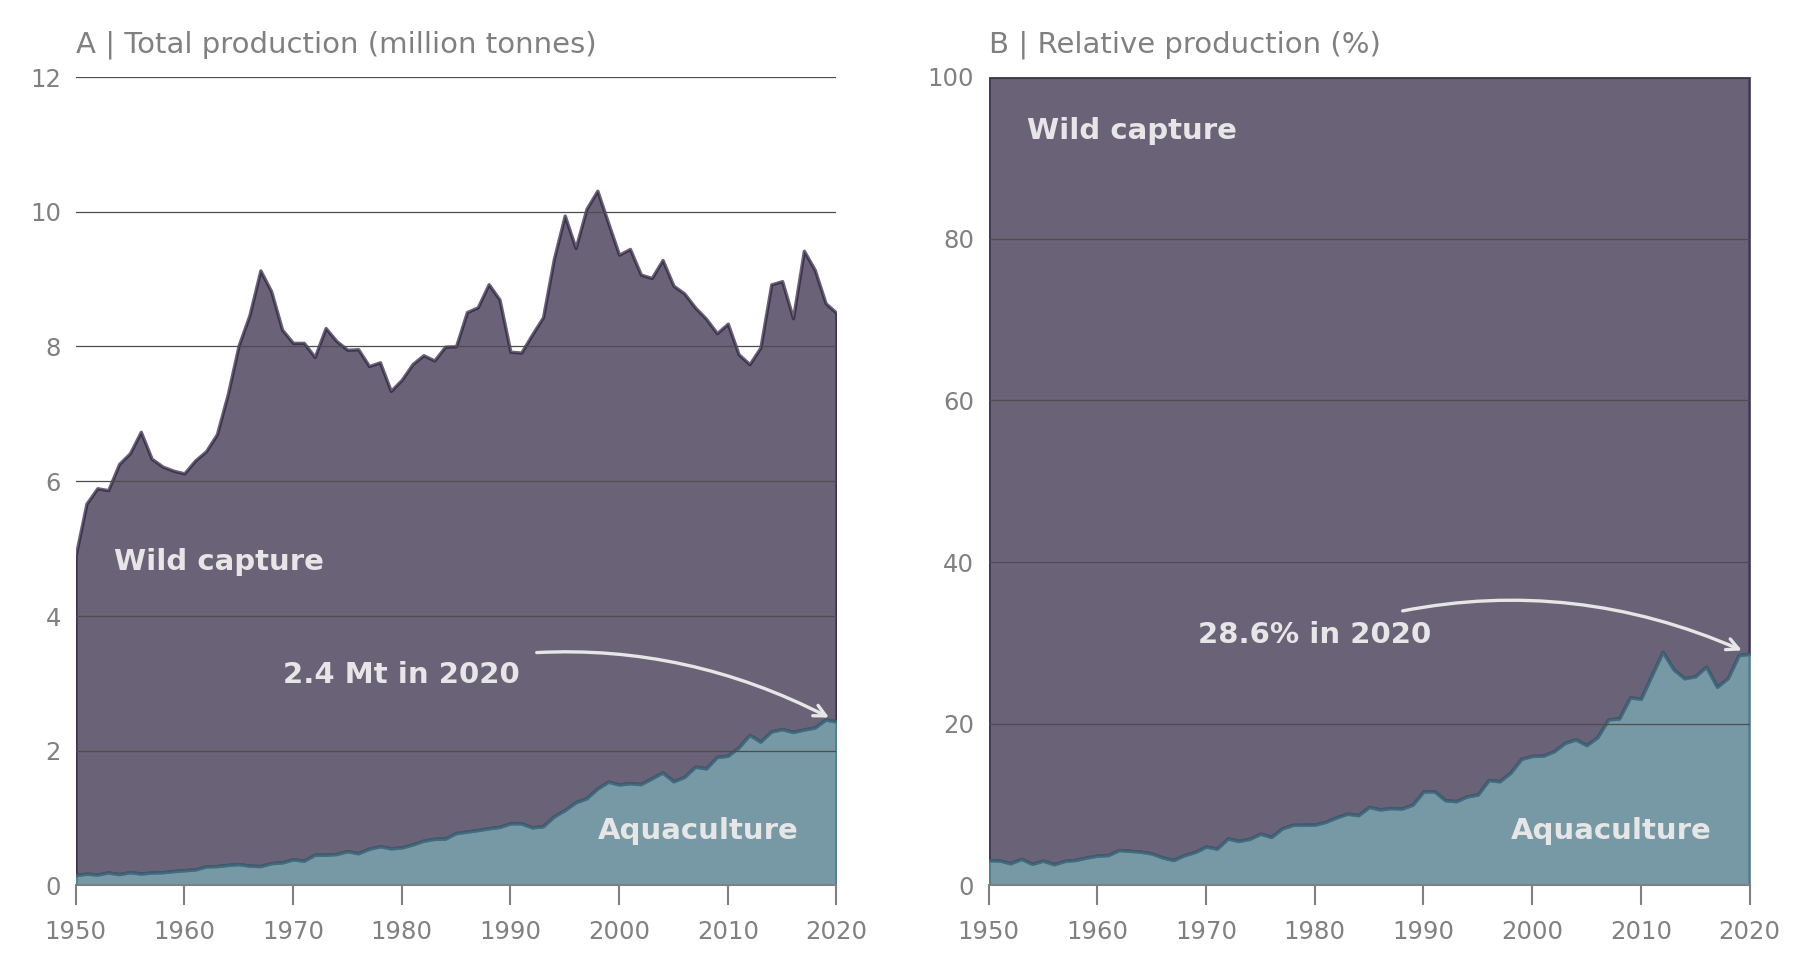
\includegraphics[width=0.95\textwidth]{production_nea_wild_capture_aquaculture}
    \caption[TBD]{TBD}
    \label{fig:TBD}
\end{figure}


\begin{figure}
    \centering
    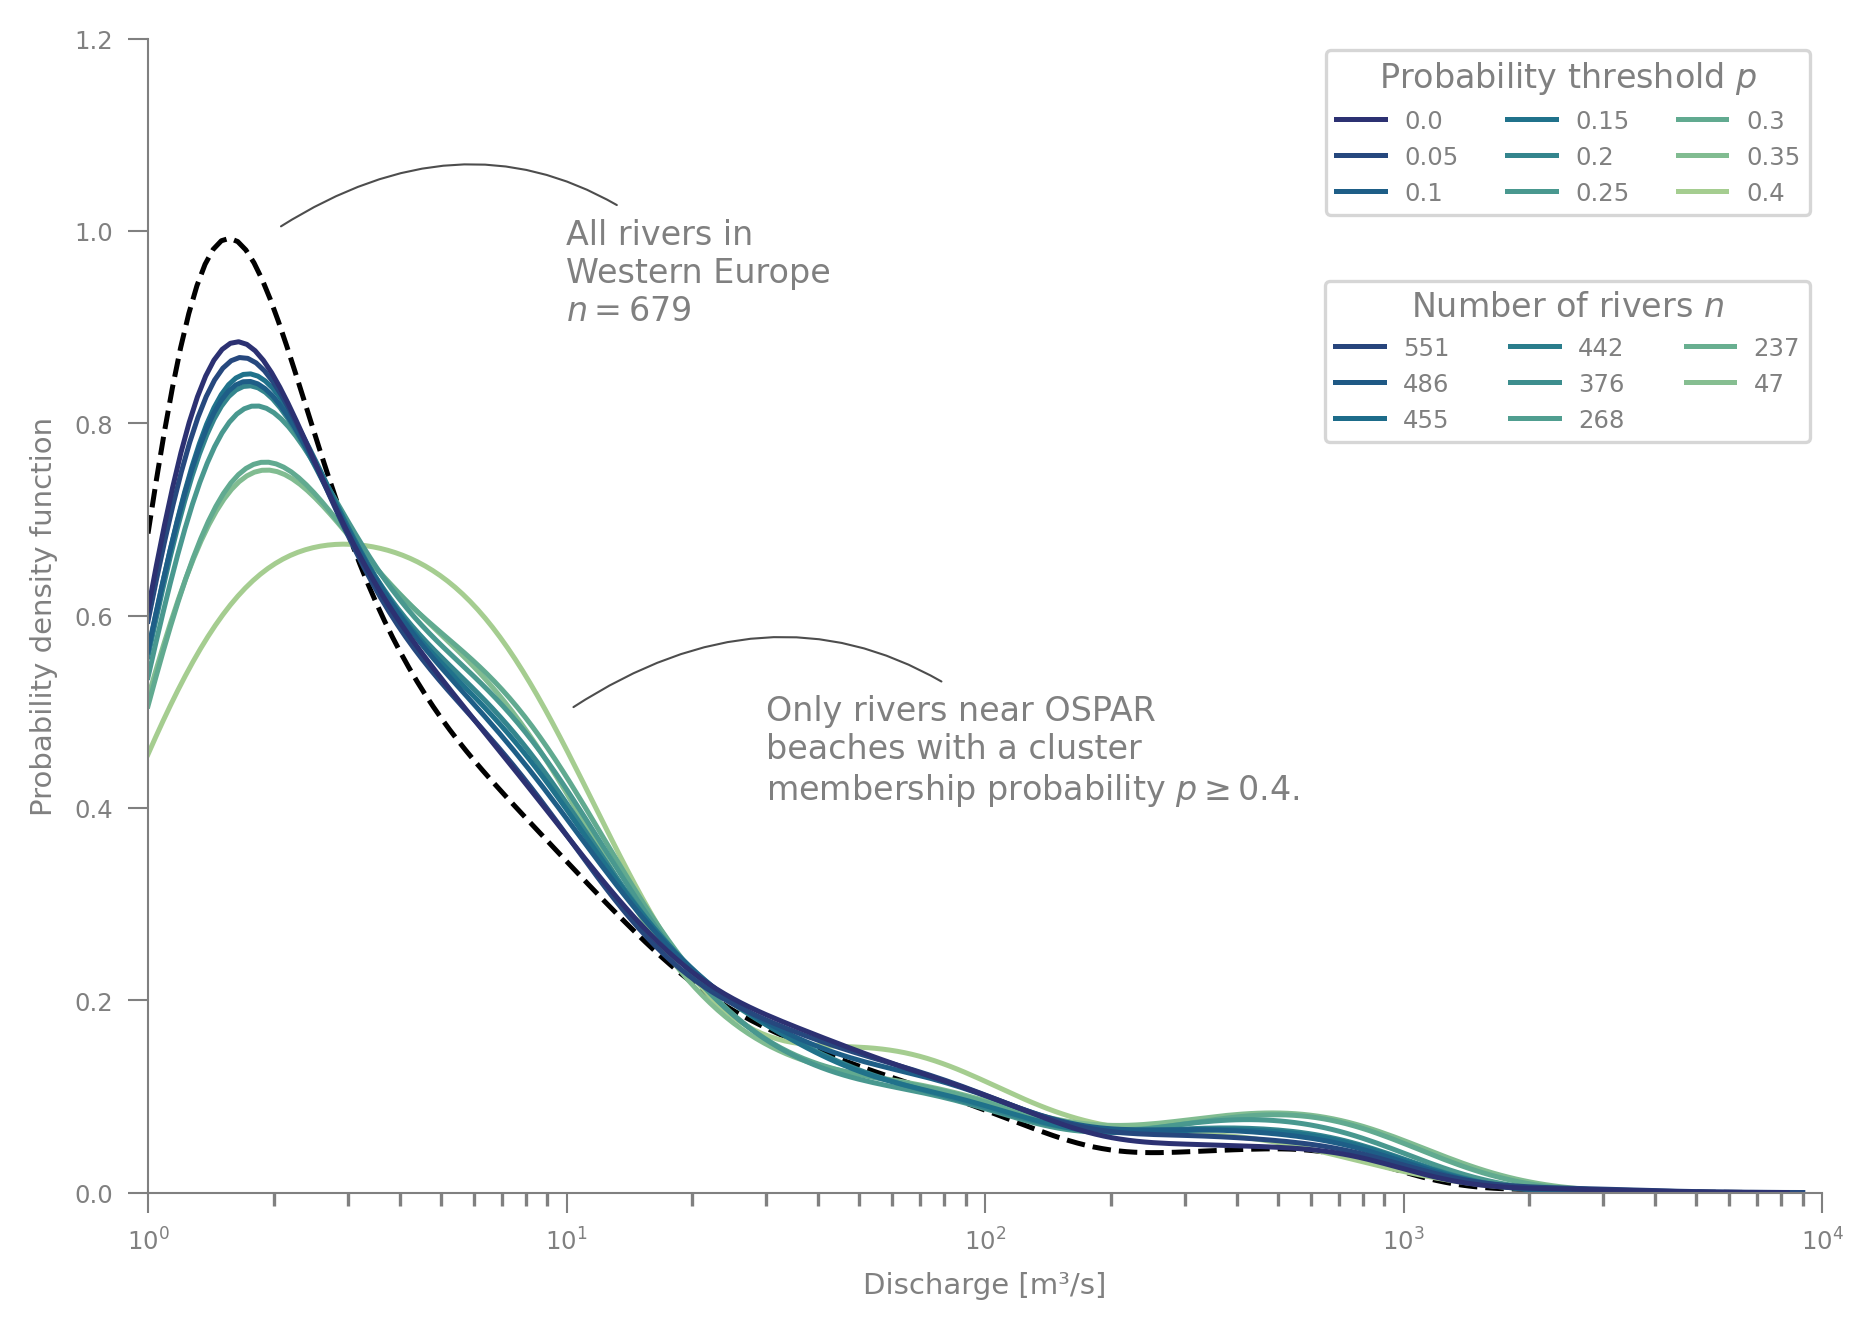
\includegraphics[width=0.95\textwidth]{river_discharge_pdfs}
    \caption[TBD]{TBD}
    \label{fig:TBD}
\end{figure}

\begin{figure}
    \centering
    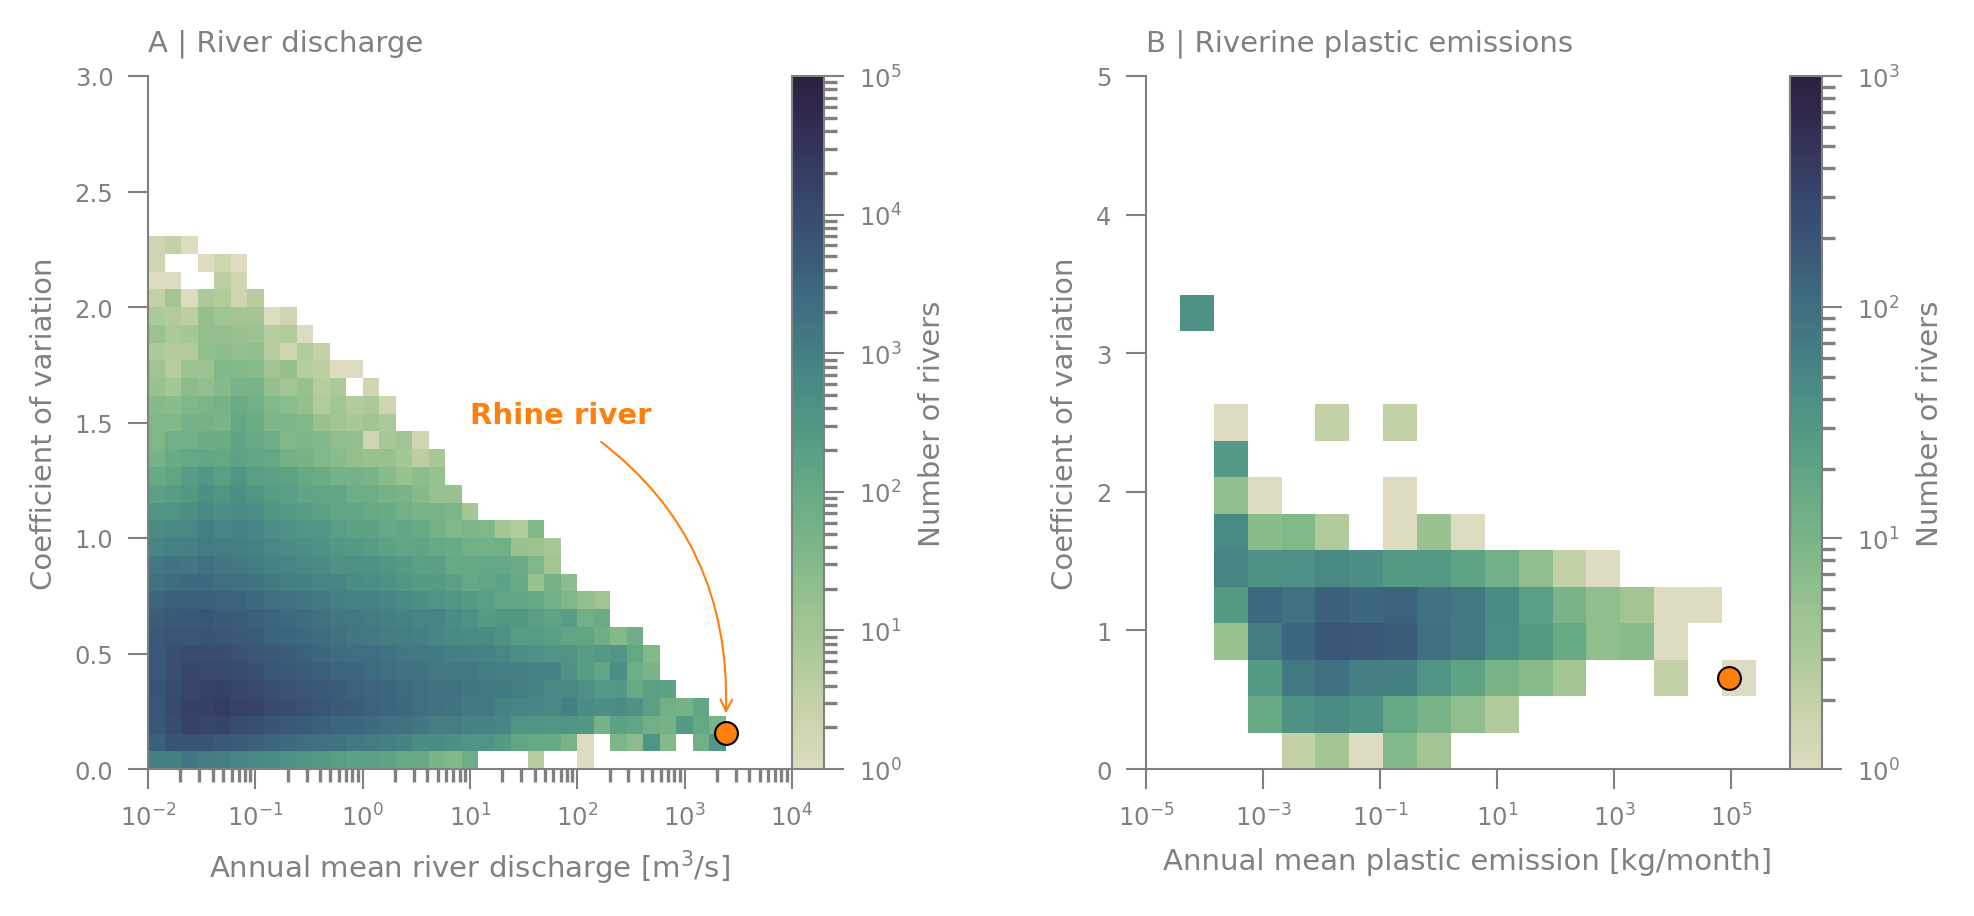
\includegraphics[width=0.95\textwidth]{river_discharge_seasonality}
    \caption[TBD]{TBD}
    \label{fig:TBD}
\end{figure}


\begin{table}[t]
    \caption{\small{Inference of parameters of the log-Gaussian Cox process model: variances $\eta_i^2$, length scales $\rho_i$ measured in \unit{km}, with $i\in\{\text{short}, \text{long}\}$, spatial mean $\mu_{\mu}$ and over-dispersion $\phi$. Shown are the 50\textsuperscript{th} percentile (median) together with the 95 \% highest density interval (in parentheses) given by the minimum width Bayesian credible interval (BCI).}}
    \label{supp:tab:model_parameter_posterior}
    \footnotesize
    \centerline{
        \begin{tabular}{@{}lllllll@{}}
            \toprule
            & $\eta_{\text{short}}^2$               & $\rho_\text{short}$         & $\eta_{\text{long}}^2$              & $\rho_{\text{long}}$            & $\mu_{\mu}$           & $\phi$               \\ \midrule
            Winter    & 1.08 (0.92; 1.23)  & 16 ( 10; 23) & 0.64 (0.33; 0.93) & 777 (236; 1965) & 184 (53; 352)  & 1.51 (1.37; 1.66) \\
            Spring    & 1.19 (1.02; 1.38)  & 16 (10; 22)  & 0.72 (0.42; 1.04) & 508 (215; 1097) & 232 (79; 440) & 1.36 (1.25; 1.48) \\
            Summer    & 1.08 (0.94; 1.24)  & 12 (7; 17)   & 0.65 (0.36; 0.97) & 593 (206; 1452) & 154 (56; 290)  & 1.54 (1.41; 1.68) \\
            Autumn    & 1.06 (0.93; 1.21) & 9 (6; 13)    & 0.60 (0.33; 0.90) & 690 (227; 1934) & 174 (73; 332)  & 1.53 (1.41; 1.66) \\ \bottomrule
        \end{tabular}
    }
    
\end{table}



\begin{table}[t]
    \centering
    \caption{\small{Median relative difference of macroplastic $X$ between season $i$ and $j$ computed as $\mathrm{med}\left((X_j - X_i)/X\right)$ where  $X = X_i$ if $\mathrm{med}(X_j - X_i) \geq 0$, else $X = X_j$. Here, $\mathrm{med}(\cdot)$ refers to the median. We then computed estimates for the NEA region as weighted median over all beaches with the individual confidence estimates as weights. For simplicity, all values are shown in percentage, together with their 25\textsuperscript{th} and 75\textsuperscript{th} weighted percentile.}}
    \label{supp:tab:seasonal_effect_size_ci}
    \begin{tabular}{c|cccc}
        $\leq$ & \textbf{Winter}  & \textbf{Spring} & \textbf{Summer} & \textbf{Autumn} \\
        \midrule
        \textbf{Winter} & - & $88(34;238)$ & $78(38;160)$  & $60(32;184)$ \\
        \textbf{Spring} & $90(49;190)$ & - & $75(38;185)$ & $72(38;223)$ \\
        \textbf{Summer} & $108(66;204)$ & $108(53;202)$ & - & $80(45;121)$ \\
        \textbf{Autumn} & $95(48;182)$ & $118(58;243)$ & $61(26;123)$ & - \\
    \end{tabular}
\end{table}

\subsection{Identification of Seasonal Hotspots}

Our analysis reveals that seasonal variations in plastic pollution are not uniformly distributed but are spatially clustered, exhibiting stark differences across various European coastal regions (Figure~\ref{fig01}). Notably, the western Iberian Peninsula, the western French coastline, the Irish Sea, and the Skagerrak exhibit strong seasonal patterns. Conversely, the North Sea region displays relatively low seasonal beach litter variations. By comparing standardized variance of macroplastic with the seasonal effect size on a per-beach level, we identified a strong correlation ($+0.60$), suggesting that the observed variability in OSPAR beach pollution levels can be partially attributed to seasonal factors (Supplementary Figure~2). 

To further explore these observations, we employed Principal Component Analysis (PCA)-driven clustering to discern underlying seasonal variation patterns (see Methods~\ref{sec:methods:clustering}). This analysis yielded two principal clusters indicative of distinct seasonal behaviors (Figure~\ref{fig03}):

\begin{itemize}
    \item \textbf{Cluster $C1^+$} is characterized by a marked increase in plastic pollution during \textbf{spring}, predominantly observed in the Skagerrak and, to a lesser extent, along the French and Iberian western coastlines.
    \item \textbf{Cluster $C2^+$} exhibits heightened plastic abundance in the \textbf{winter/spring} seasons, spatially similar to cluster $C1^+$, strongly influenced by beaches along the western Iberian and French coastlines and around the Irish Sea.
\end{itemize}

Both clusters highlight a comparative increase in pollution during the winter/spring months over summer/autumn, a pattern reported in previous studies for these specific regions \cite{svard_analys_2013,kanstrup_plastic_2018,le_moigne_cleanatlantic_2021, gago_characteristics_2014,declerck_transport_2019,ruiz_modelling_2022,schulz_multi-criteria_2013}. However, our clustering supports the notion that even within these regions, beaches with different seasonal patterns than those reported as dominant may occur, indicating high spatial variability on small scales. This variability may explain the divergent findings in some studies \cite{schulz_multi-criteria_2013,gago_characteristics_2014,watts_through_2017,rios_spatio-temporal_2018,asensio-montesinos_seasonal_2019,ruiz_modelling_2022}.

Utilizing our PCA-derived cluster weights alongside LGCP-modeled beach litter distributions, we calculated weighted percentiles for each cluster, revealing substantial seasonal differences (Figure~\ref{fig04}). For instance, the cluster $C1^+$ shows median pollution levels escalating from 207 \itm in autumn to 643 \itm in spring. This springtime peak signifies a more than 200\% increase in median plastic pollution levels compared to autumn, identifying a strong seasonal hotspot. 

Conversely, winter/spring cluster $C2^+$ presents a more uniform distribution between seasons, with the most considerable relative increase observed as a 150\% rise in winter compared to summer. This pattern suggests that cluster $C2^+$ more closely represents the general seasonal trend across European beaches, whereas $C1^+$ captures regions with more extreme seasonal fluctuations.

These seasonal pollution levels are well above the European Union threshold value (EU TV) of 20 \itm for beach litter \cite{van_loon_european_2020}, underscoring the urgent need for targeted litter management strategies. Specifically, our results for cluster $C1^+$ indicate that relying on annual medians as a measure of beach litter pollution, which suggests a pollution level of 274 \itm in agreement with previous research \cite{schulz_baseline_2019,hanke_eu_2019, van_loon_european_2020,lacroix_abundance_2023}, can be misleading as it fails to account for seasonal pollution peaks.



\subsection{Drivers of Seasonal Hotspots in Anthropogenic Beach Litter}

To illuminate the origins of the identified seasonal hotspots for beach litter in the NEA, particularly during spring ($C1^{+}$) and winter/spring ($C2^{+}$), we examined the relationship between these hotspots and the global sources of marine litter: riverine macroplastic emissions \cite{lebreton_river_2017,meijer_more_2021,strokal_river_2023,kaandorp_global_2023, zhang_plastic_2023, gonzalez-fernandez_floating_2021}, fishing \cite{kroodsma_tracking_2018,kaandorp_global_2023,paolo_satellite_2024} and aquaculture activities \cite{tian_can_2022, skirtun_plastic_2022,kruger_plastic_2020,paolo_satellite_2024}.

We analyzed the latest data on simulated riverine emissions of macrolitter \cite{strokal_river_2023}. Given that these data represent average annual emissions, we employed high-resolution reanalysis data of river discharge to infer seasonal variation \cite{mazzetti_reforecasts_2023}, approximating the amount of macroplastics entering the ocean from rivers at different times of the year (Methods \ref{sec:methods:seasonal_potential}).

To assess the impact of fishing-related activities, we utilized high-resolution daily data on fishing intensity \cite{kroodsma_tracking_2018}. For estimating seasonal variations in local litter emissions from mariculture, we employed a recently developed dataset of mariculture production locations \cite{clawson_mapping_2022}, combining it with seasonal information derived from changes in mean monthly ocean wave energies as a proxy for adverse weather conditions \cite{skirtun_plastic_2022,global_ghost_gear_initiative_best_2021} (Methods \ref{sec:methods:seasonal_potential}, Supplementary Figure~3). Additionally, to enhance our analysis, we proposed two alternative scenarios for the seasonality of mariculture production: one using monthly national export statistics and the other using river discharge data for farms situated in rivers \cite{rocha_global_2022}.

To quantify each source's potential to create the observed seasonal beach litter patterns, we calculated both the coefficient of variation ($c_{\text{v}}$) and the Pearson correlation coefficient ($c_{\text{r}}$) of monthly climatologies. The former measures the magnitude of seasonal variations, while the latter indicates the degree of similarity between the seasonal variations of beach litter and litter sources. We then introduced a seasonal potential metric ($\Phi$), calculated as $\Phi = \max (c_{\text{v}}c_{\text{r}}, 0)$, which identifies the strongest seasonal signals in the potential sources of beach litter, prioritizing those with strong variability and temporal alignment with the observed litter patterns (Methods~\ref{sec:methods:seasonal_potential}).

Our analysis revealed that both riverine discharge and mariculture exhibit a strong seasonal potential $\Phi$ to explain the seasonal variations in beach litter during the winter/spring pattern (Figure~\ref{fig05}).  In contrast, fisheries display a low seasonal potential, close to zero (Figure~\ref{fig05}C-D), due to relatively minor seasonal variations that typically peak during summer in most regions. This indicates that fisheries are less likely to substantially contribute to seasonal beach litter variations. Furthermore, since less than $5\%$ of wild capture occurs within the first 4 km of the coastline--with the majority happening tens of kilometers offshore (Supplementary Figure~4)--macroplastic emissions from fishing vessels are likely to diffuse over space and time \cite{sebille_physical_2020}.

Interestingly, our findings suggest that numerous small-scale rivers (annual mean discharge $\sim 10$~$m^3s^{-1}$), rather than larger ones, are more likely responsible for the observed seasonal variations (Figure~\ref{fig05}A-B, Supplementary Figure~5). Smaller rivers tend to exhibit more pronounced seasonal fluctuations than larger rivers (Supplementary Figure~6), underscoring their importance as pathways for macroplastics from continental to marine environments \cite{gonzalez-fernandez_floating_2021}. Our analysis supports previous studies indicating that major rivers are minor contributors to floating litter variability in the North Sea \cite{thiel_spatio-temporal_2011}, where the potential influence of large river systems like the Rhine is comparatively low (Figure~\ref{fig05}A-B, Supplementary Figure~6).

To further investigate the drivers of seasonal variations, we computed the relative fractions of plastic items likely linked to land, fishing or mariculture activities (Methods~\ref{sec:methods:ospar}). This analysis aimed to determine if the seasonal patterns observed in absolute item counts could be explained by an increase in the relative fraction of these three sources. We modeled the fraction for each source and season separately using Gaussian Processes in the logit-transformed space. Subsequently, we performed PCA-clustering for each source, similar to the approach used in Figure~\ref{fig03}, resulting in one significant cluster per source.

By examining these clusters, we found that only the mariculture-related items displayed a winter/spring pattern similar to cluster $C2^{+}$ of the absolute item counts (Figure~\ref{fig03}, Supplementary Figure~7). Additionally, the spatial pattern of mariculture-related items largely aligns with the identified hotspots along the western Iberian and French coastlines. This suggests that an increase in mariculture-related items could partially explain the rise in absolute item counts during winter/spring. In contrast, the temporal and spatial patterns of clusters derived from land and fisheries fractions did not match any cluster patterns found for absolute item counts. While there is a growing number of studies noting the importance of plastic emissions from mariculture systems \cite{kruger_plastic_2020,tian_can_2022,skirtun_plastic_2022}, not much is known about their seasonality. Previous results from mariculture-exposed sandy beaches along the coast of Chile suggest considerable seasonality of fishing/mariculture-related items \cite{thiel_anthropogenic_2013}. More recently, pronounced seasonal variations in the abundance of microplastics were found in a predominantly bivalve-mariculture-influenced bay in Thailand \cite{ruangpanupan_seasonal_2023}.

To test whether bivalve aquaculture in the NEA provide a potential source of beach litter variability, we computed the seasonal potential specifically for bivalves/invertebrates (mainly mussels and oysters farming in the NEA). The results were very similar to those for all mariculture production (Supplementary Figure~8,~9). The primary difference is that bivalves/invertebrates production is less concentrated along the Norwegian coastline, which is predominantly salmon mariculture \cite{fao_state_2022}. This difference better matches the observed seasonal patterns of beach litter; however, it is not entirely conclusive due to the relatively low number of surveyed beaches in that area, complicating validation.

It is important to note that not all items can be confidently linked to these specific sources, as $60.1 \%$ of items found in the NEA have degraded to the point where they are unrecognizable and are categorized generically (e.g. "large plastics" or "others"; see Methods~\ref{sec:methods:ospar}). These low numbers of identifiable items likely reduce the confidence in the model's ability to detect certain patterns (Supplementary Figure~7).

Additionally, our study makes a few key simplifications. Firstly, our approach assumes that seasonal variations in macroplastics is mainly due to local sources, while the impact of more distant sources is negligible. Although simulation studies show that plastics can travel vast oceanic distances and in some cases remote contributions can outweigh local ones \cite{chassignet_tracking_2021, chenillat_fate_2021,onink_global_2021}, recent studies indicated that coastal areas mainly accumulate locally sourced macroplastics \cite{morales-caselles_inshoreoffshore_2021}. Furthermore, our own analysis suggests that there are hardly coherent spatial structures on length scales beyond 100 km (Supplementary Notes~2, Supplementary Table~1). This leads us to believe the impact of distant plastics on our findings is minimal.

Secondly, our analysis overlooks ocean dynamics and their role in distributing plastics \cite{sebille_physical_2020}, which may cause seasonal variations in beach litter independent of the original source's constancy. We posit that, given the predominance of local sources for beach macroplastics in Europe, ocean transport effects are secondary, though exceptions may exist \cite{neumann_marine_2014}.

Lastly, while methods are available to trace beach litter back to its sources \cite{van_duinen_identifying_2022, pierard_attribution_2022}, they rely on knowing each source's relative contribution, challenging to determine for fish capture versus mariculture \cite{skirtun_plastic_2022}. Global estimates on source shares exist  \cite{lebreton_evidence_2018,kaandorp_global_2023}, but regional data may vary greatly \cite{bringer_coastal_2021,morales-caselles_inshoreoffshore_2021, strokal_river_2023}. The tracking of fishing activity is feasible through automatic identification system positions \cite{kroodsma_tracking_2018}, yet our understanding of the timing and scale of plastic emissions from mariculture remains limited \cite{paolo_satellite_2024,tian_can_2022}.



\section{Conclusion}\label{sec:beach_litter:conclusion}
Our study provides evidence that seasonal variations in macroplastics pollution on beaches in the NEA are more important than previously recognized \cite{schulz_multi-criteria_2013}. Emissions from numerous small-scale rivers and mariculture-related activities, likely driven by seasonally dependent adverse weather conditions -- conditions projected to increase in the future \cite{konisky_extreme_2016} -- may be key contributors. With aquaculture production in the NEA having surged by approximately 117\% over the last two decades \cite{ospar_comission_feeder_2021,fao_state_2022} (Supplementary Figure~10), the role of this sector in contributing to beach litter is expected to grow \cite{bringer_coastal_2021,skirtun_plastic_2022,kruger_plastic_2020,tian_can_2022}. While Regulation (EU) 2021/1139 marks progress towards sustainable mariculture within the EU, our study underscores the urgent need for more specific and effective strategies to address mariculture-related plastic emissions.

Addressing the complexities of beach litter, particularly from mariculture, requires a comprehensive enhancement of the existing monitoring network. The Marine Strategy Framework Directive (MSFD) Technical Group on Marine Litter recommends that beach litter assessments be conducted seasonally \cite{galgani_guidance_2023}, i.e., four times a year, to capture the fluctuating dynamics of litter accumulation. Our findings support this recommendation, highlighting the importance of sufficient temporal resolution in monitoring to effectively identify and address seasonal litter hotspots. Furthermore, a more refined categorization of litter items is necessary to confidently identify litter sources \cite{ospar_comission_feeder_2021}. Recent studies have shown that using OSPAR categorization can underestimate actual mariculture-related items by a factor of four \cite{skirtun_plastic_2022}. Accurate categorizations would also provide a robust basis for informing probabilistic Lagrangian backward simulations \cite{van_duinen_identifying_2022, pierard_attribution_2022} needed to identify sources considering ocean currents.

Our research also identifies strategic opportunities for more efficient removal of macroplastics from beaches by focusing efforts on regions and periods identified as seasonal hotspots. Additionally, the collection of large items from beaches serves as a useful stopgap measure to limit the formation of microplastics while effective steps to prevent plastic leakage into the environment are formulated \cite{ryan_toward_2020}. For example, targeted cleanup operations in the Skagerrak during spring and along the French and Iberian western coastlines throughout winter and spring could enhance the efficiency of litter collection efforts. Such focused initiatives could potentially double the median quantity of items collected, providing valuable insights for NGOs and citizen science projects aimed at maximizing environmental impact, enhancing community engagement, and raising public awareness about marine litter issues. Furthermore, involving citizen science in monitoring efforts presents a promising approach to supplement traditional data collection methods \cite{conrad_review_2011,hidalgo-ruz_contribution_2015}.

In addition to better quantifying plastic emissions from mariculture \cite{tian_can_2022}, addressing the root causes of macroplastic leakage into the marine environment is paramount. Our study emphasizes the importance of adhering to policy recommendations made by the Aqua-Lit project \cite{hipolito_policy_2020}, which include using high-quality materials in mariculture installations, expanding waste collection, and implementing protocols for monitoring plastic waste. These efforts should be complemented by incentives such as quality seals and bonuses for adherence to sustainable practices \cite{redacuiculturaplastic_creacion_2022, skirtun_plastic_2022}. The advancement of extended producer responsibility schemes \cite{leal_filho_overview_2019} further supports these initiatives.